%%%%%%%%%%%%%%%%%%%%%%%%%%%%%%%%%%%%%%%%%
% Short Sectioned Assignment LaTeX Template Version 1.0 (5/5/12)
% This template has been downloaded from: http://www.LaTeXTemplates.com
% Original author:  Frits Wenneker (http://www.howtotex.com)
% License: CC BY-NC-SA 3.0 (http://creativecommons.org/licenses/by-nc-sa/3.0/)
%%%%%%%%%%%%%%%%%%%%%%%%%%%%%%%%%%%%%%%%%

%----------------------------------------------------------------------------------------
%	PACKAGES AND OTHER DOCUMENT CONFIGURATIONS
%----------------------------------------------------------------------------------------

\documentclass[paper=a4, fontsize=11pt]{scrartcl} % A4 paper and 11pt font size
% ---- Entrada y salida de texto -----

\usepackage[T1]{fontenc} % Use 8-bit encoding that has 256 glyphs
\usepackage[utf8]{inputenc}
%\usepackage[default]{sourcesanspro}
\usepackage{fourier} % Use the Adobe Utopia font for the document - comment this line to return to the LaTeX default
% ---- Idioma --------

\usepackage[spanish, es-tabla]{babel} % Selecciona el español para palabras introducidas automáticamente, p.ej. "septiembre" en la fecha y especifica que se use la palabra Tabla en vez de Cuadro

% ---- Code insertion ----
\usepackage{minted}
\usepackage[breakable]{tcolorbox} %Genera boxes, lo usamos para el codigo
\BeforeBeginEnvironment{minted}{\begin{tcolorbox}[breakable]}%
	\AfterEndEnvironment{minted}{\end{tcolorbox}}%
\BeforeBeginEnvironment{inputminted}{\begin{tcolorbox}[breakable]}%
	\AfterEndEnvironment{inputminted}{\end{tcolorbox}}%

\usepackage{xpatch} %permite abrir environments al ejecutar ciertos comandos

\xpretocmd{\inputminted}{\begin{tcolorbox}}{}{}%
	\xapptocmd{\inputminted}{\end{tcolorbox}}{}{}%

\setminted{
fontsize=\small,
breaklines,
breaksymbolleft=
}
% ---- Otros paquetes ----
\usepackage{dirtree}
\usepackage{vmargin}

\usepackage{url} % ,href} %para incluir URLs e hipervínculos dentro del texto (aunque hay que instalar href)
\usepackage{hyperref} % ,href} %para incluir URLs e hipervínculos dentro del texto (aunque hay que instalar href)
\hypersetup{
	colorlinks=true,
	linkcolor=blue,
	filecolor=magenta,      
	urlcolor=blue,
}

\usepackage{xcolor}
\definecolor{light-gray}{gray}{0.95}
\definecolor{alizarin}{rgb}{0.82, 0.1, 0.26}
\definecolor{nyellow}{rgb}{0.91, 0.656, 0.0}
%\definecolor{indigo}{rgb}{0.29, 0.0, 0.51}
%	\textcolor{red}{p}
%	\textcolor{orange}{r}
%	\textcolor{yellow}{a}
%	\textcolor{green}{c}
%	\textcolor{blue}{t}
%	\textcolor{indigo}{i}
%	\textcolor{violet}{c}
%	\textcolor{red}{a}
%	\textcolor{orange}{s}
%	\textcolor{yellow}{,}
%	\textcolor{green}{I}
%	\textcolor{blue}{S}
%	\textcolor{indigo}{E}

\usepackage{amsmath,amsfonts,amsthm} % Math packages
%\usepackage{graphics,graphicx, floatrow} %para incluir imágenes y notas en las imágenes
\usepackage{graphics,graphicx, float} %para incluir imágenes y colocarlas
\usepackage[export]{adjustbox}
\graphicspath{{imagenes/}}

% Para hacer tablas comlejas
%\usepackage{multirow}
%\usepackage{threeparttable}

%\usepackage{sectsty} % Allows customizing section commands
%\allsectionsfont{\centering \normalfont\scshape} % Make all sections centered, the default font and small caps

%Remove warnings
\usepackage{silence}
\WarningFilter{scrartcl}{Usage of package `fancyhdr'}

\usepackage{fancyhdr} % Custom headers and footers
\pagestyle{fancyplain} % Makes all pages in the document conform to the custom headers and footers
\fancyhead{} % No page header - if you want one, create it in the same way as the footers below
\fancyfoot[L]{} % Empty left footer
\fancyfoot[C]{} % Empty center footer
\fancyfoot[R]{\thepage} % Page numbering for right footer
\renewcommand{\headrulewidth}{0pt} % Remove header underlines
\renewcommand{\footrulewidth}{0pt} % Remove footer underlines
\setlength{\headheight}{13.6pt} % Customize the height of the header

\numberwithin{equation}{section} % Number equations within sections (i.e. 1.1, 1.2, 2.1, 2.2 instead of 1, 2, 3, 4)
\numberwithin{figure}{section} % Number figures within sections (i.e. 1.1, 1.2, 2.1, 2.2 instead of 1, 2, 3, 4)
\numberwithin{table}{section} % Number tables within sections (i.e. 1.1, 1.2, 2.1, 2.2 instead of 1, 2, 3, 4)

\setlength\parindent{0pt} % Removes all indentation from paragraphs - comment this line for an assignment with lots of text

\newcommand{\horrule}[1]{\rule{\linewidth}{#1}} % Create horizontal rule command with 1 argument of height

\setmarginsrb{2 cm}{1 cm}{2 cm}{2 cm}{1 cm}{1.5 cm}{1 cm}{1.5 cm} %Aumenta los márgenes

%----------------------------------------------------------------------------------------
%	TÍTULO Y DATOS DEL ALUMNO
%----------------------------------------------------------------------------------------

\title{
	Práctica 2.b \\\vspace{1cm}
	Técnicas de Búsqueda Local y Algoritmos Greedy
	para el Problema del Aprendizaje de Pesos en
	Características \vspace{1cm} \\
	El problema del Aprendizaje de Pesos en Características (APC)	\vspace{1cm} \\
	Algoritmos Genéticos \\
	Algoritmos Meméticos \hspace{1cm} 
 }   

\author{Yeray López Ramírez	}                             

\renewcommand*\contentsname{hola}

\makeatletter
\let\thetitle\@title
\let\theauthor\@author
\let\thedate\@date
\makeatother

%----------------------------------------------------------------------------------------
% DOCUMENTO
%----------------------------------------------------------------------------------------

\begin{document}
\begin{titlepage}
	\centering
	%\textsc{\LARGE Universidad de Granada}\\[2.0 cm]    
	
\includegraphics[scale = 0.6]{ugr.png}\\[1.0 cm]
	\rule{\linewidth}{0.2 mm} \\[0.4 cm]
	{ \huge \bfseries \thetitle}\\
	\rule{\linewidth}{0.2 mm} \\[1.5 cm]
	
	\begin{minipage}{0.5\textwidth}
		\begin{flushleft} \large
			\theauthor 
			123456789-Z \\
			\href{mailto:fulanito@correo.ugr.es}{fulanito@correo.ugr.es}
		\end{flushleft}
	\end{minipage}~
	\begin{minipage}{0.5\textwidth}
		\begin{flushright} \large
			Curso: 2022-23 \\
			Grupo A, 15:30 - 17:30 (Martes)                   
		\end{flushright}
	\end{minipage}\\[1 cm]
	
	{\small \thedate}\\[1 cm]
	
	\vfill
	
\end{titlepage}


\newpage %inserta un salto de página
\newcommand{\code}[1]{\colorbox{light-gray}{\textcolor{alizarin}{\texttt{#1}}}}
\newcommand{\high}[1]{\colorbox{light-gray}{\textcolor{nyellow}{\texttt{#1}}}}

\tableofcontents % para generar el índice de contenidos

\listoffigures

\listoftables

\newpage

%----------------------------------------------------------------------------------------
%	Cuestión 1
%----------------------------------------------------------------------------------------

\section{Descripción del problema}
El problema del Aprendizaje de Pesos en Características (APC) consiste en encontrar una combinación ponderada de un conjunto de características que maximice la precisión de un clasificador y minimice su complejidad. En este problema, se busca determinar la importancia relativa de cada característica para mejorar la eficiencia computacional y la precisión del modelo. El objetivo es encontrar un vector de pesos que asigne valores más altos a las características más importantes y valores más bajos a las características menos relevantes, y que permita eliminar aquellas características que no aporten información relevante para la tarea de clasificación. \\

En otras palabras, el APC busca determinar qué características son más relevantes para un problema dado y cómo combinarlas de manera óptima para obtener el mejor rendimiento de un modelo. \\

El modelo clasificador utilizado en este problema es el 1-NN, el cual es un método de aprendizaje supervisado que clasifica una instancia basándose en la clase de su vecino más cercano en el conjunto de entrenamiento. Además, se utilizará la técnica de validación leave-one-out para evaluar el desempeño del clasificador. La función objetivo que se busca maximizar será una combinación de medidas de precisión (tasa\_clas) y complejidad del clasificador (tasa\_red), dando como resultado el fitness.\\

Los conjuntos de datos utilizados en este problema son \textbf{diabetes}, \textbf{ozone-320} y \textbf{spectf-heart}. Diabetes es un conjunto de datos médicos que contiene información sobre pacientes con diabetes, como su edad, índice de masa corporal, presión arterial y resultados de pruebas de laboratorio, entre otros. Ozone-320 es un conjunto de datos de calidad del aire que contiene mediciones de ozono y otros contaminantes atmosféricos en diferentes ciudades de Estados Unidos. Spectf-heart es un conjunto de datos médicos que contiene información sobre pacientes que se sometieron a pruebas de diagnóstico por imágenes para enfermedades cardíacas. Todos los datasets tienen 2 etiquetas: negativo/positivo o 1.0/2.0 para indicar la clase del vector de características.  
\newpage

\section{Descripción de la aplicación de los algoritmos}
Los algoritmos utilizados para resolver el problema del Aprendizaje de Pesos en Características (APC) son Metaheurísticas que buscan optimizar una función objetivo que combina la precisión y la complejidad del clasificador 1-NN diseñado utilizando un vector de pesos. En este problema, se busca encontrar el mejor subconjunto de características que permita obtener una alta tasa de clasificación y, al mismo tiempo, reducir la complejidad del modelo. \\

Para aplicar estos algoritmos al problema de APC, se utilizó el esquema de representación basado en un vector de tamaño n con valores en [0, 1] que indican el peso asociado a cada característica. La función objetivo fue definida como la combinación con pesos de la tasa de acierto y la tasa de reducción de características del clasificador 1-NN diseñado empleando el vector de pesos. El objetivo es maximizar esta función, multiplicando la tasa de acierto por 0.8 y la tasa de reducción por 0.2, para dar mayor importancia a la clasificación que a la reducción de características.
\[\text{Fit} = 0.8 \cdot \text{precision} + 0.2 \cdot \text{reduction}\]

La implementación en pseudocódigo de la \textbf{función objetivo}:

\begin{minted}{text}
Input(Conjunto de Entrenamiento "Train", Conjunto de Prueba "Test", Vector de pesos W)
Inicio
    aciertos <- CLASIFICAR(Train, Test, W)
    tasa_clas <- aciertos/tamaño_test
    tasa_red <- PESOS_MENOR_UMBRAL(W, 0.1)
    DEVOLVER(0.8·tasa_clas + 0.2·tasa_red)
Fin
\end{minted}

Donde CLASIFICAR llama al modelo clasificador de vecinos 1-NN. El clasificador 1-NN (del inglés "Nearest Neighbor") es un algoritmo de clasificación que se basa en encontrar el vecino más cercano a un ejemplo de prueba en un conjunto de datos de entrenamiento, y asignarle la etiqueta del vecino como la etiqueta del ejemplo de prueba. En otras palabras, el algoritmo encuentra el ejemplo de entrenamiento más cercano al ejemplo de prueba en términos de \textbf{distancia}, y le asigna la etiqueta del ejemplo de entrenamiento como la etiqueta del ejemplo de prueba. La implementación en pseudocódigo del \textbf{clasificador 1NN} es:

\begin{minted}{c++}
Input(Vector características "A", Conjunto Entrenamiento "T", pesos W)
Inicio
    Inicializar min_distancia(INFINITY) y min_index(-1)
    Para cada vector B en T
        distancia <- DISTANCIA_EUCLIDEA(A,B,W)
        Si distancia es menor que min_distancia
            entonces min_index <- T.indice y min_distancia <- distancia
     DEVOLVER(T.GET_ETIQUETA(min_index))
Fin
\end{minted}

Cuando la función objetivo llama a CLASIFICAR lo que realmente hace es ejecutar el clasificador 1-NN con todo el conjunto de prueba. \\

Tanto el clasificador como el algoritmo de Greedy y la Búsqueda Local requieren del cálculo de la distancia entre los ejemplos. La \textbf{distancia euclidiana} es una medida de distancia comúnmente utilizada en problemas de clasificación y agrupamiento. Esta distancia mide la distancia geométrica entre dos puntos en un espacio n-dimensional. Se calcula como la raíz cuadrada de la suma de las diferencias al cuadrado de cada coordenada:

\[d(p,q) = \sqrt{(e^1_1 - e^1_2)^2 + (e^2_1 - e^2_2)^2 + ... + (e^n_1 - e^n_2)^2} =  \sqrt{\sum_{i=1}^n (e^i_1 - e^i_2)^2}\]

En el contexto del clasificador 1-NN, la distancia euclidiana se utiliza para medir la similitud entre dos ejemplos, uno del conjunto de entrenamiento y otro del conjunto de prueba. La idea es comparar el ejemplo de prueba con cada uno de los ejemplos de entrenamiento, y seleccionar la etiqueta del ejemplo más cercano al de prueba.\\

Los pesos w se usan para ajustar la importancia de cada atributo en el cálculo de la distancia euclidiana. Si un atributo tiene un peso alto, entonces su valor tendrá un mayor impacto en la medida de distancia. Por lo tanto, es importante elegir los pesos adecuados para obtener una buena precisión de clasificación. En algunos casos, ciertos atributos pueden ser irrelevantes o redundantes, y su peso puede establecerse en cero para ignorarlos en el cálculo de la distancia. La implementación en pseudocódigo de la \textbf{distancia euclidiana ponderada}:

\begin{minted}{c++}
Input(Vector características "A", Vector características "B", Vector de pesos "W", Umbral=0.1)
Inicio
    Inicializa distancia(0)
    Para cada i en número de características
        Si el peso wi es menor al umbral
            salta la iteración
        Sino
            entonces dist <- wi + (Ai - Bi)²
      DEVUELVE(RAIZ_CUADRADA(dist))
Fin
\end{minted}

Y por último pero no menos el importante, la función de \textbf{leave one out}. El Leave One Out es un procedimiento para evaluar la capacidad predictiva de un modelo de clasificación utilizando todo el conjunto de datos para el entrenamiento y la validación. El proceso consiste en evaluar el modelo n veces, dejando un ejemplo fuera (leave one out) del conjunto de datos en cada iteración para su uso en la validación. El modelo se entrena con los n-1 ejemplos restantes y se utiliza para predecir el ejemplo que se dejó fuera. La precisión del modelo se mide mediante el número de predicciones correctas sobre el total de ejemplos que se dejaron fuera. La implementación en pseudocódigo del \textbf{LOO}:

\begin{minted}{c++}
Input(Conjunto de datos "C", Indice "i")
Inicio
    Dataset Loo <- C
    ELIMINAR_EJEMPLO(Loo, i)
    DEVOLVER(Loo)
Fin
\end{minted}


\section{Estructuras de datos y algoritmos}
\subsection{Estructura de Datos en C++}
En primer lugar, mencionar que se ha elegido el lenguaje de programación C++. Se han definido principalmente dos Estructuras que forman la base del programa:
\begin{itemize}
	\item Struct Ejemplo: contiene un vector de características y un string de etiqueta. Representa a cada individuo en los conjuntos de datos.
	\item Class Dataset: contiene un vector de Ejemplos y vector de etiquetas. Representa a todo el conjunto de datos, puede ser train o test según la lectura de los datos.
	
	\item Class Poblacion: contiene una matriz de poblacion donde cada fila representa un individuo de la misma, un vector de fitness donde guarda el valor de fitness de cada individuo y varios enteros con las posiciones al peor, segundo peor y mejor fitness.
\end{itemize}

En la lectura se aplicó el método de validación cruzada (cross-folding) para evaluar el rendimiento de los algoritmos de selección de características en el problema de Aprendizaje de Pesos en Características (APC). \\

Este método consiste en dividir el conjunto de datos en $k$ particiones de igual tamaño, donde una de las particiones se utiliza como conjunto de prueba y las $k-1$ particiones restantes se utilizan como conjunto de entrenamiento. Este proceso se repite $k$ veces, de tal manera que cada partición se utiliza exactamente una vez como conjunto de prueba. De esta forma, se obtiene una medida más robusta del rendimiento del algoritmo, ya que se evalúa el rendimiento sobre datos que no han sido utilizados para entrenar el modelo. \\

En nuestro problema se utilizó la validación cruzada con $k=5$, lo que significa que se dividieron los datos en 5 particiones de igual tamaño y se realizaron 5 iteraciones del proceso de entrenamiento y evaluación. Para cada iteración, se utilizó una partición diferente como conjunto de prueba y las demás particiones como conjunto de entrenamiento. Se promedió el rendimiento obtenido en las 5 iteraciones para obtener una medida general del rendimiento de cada algoritmo. \\

Para ayudar a la reproducibilidad y verificación de los algoritmos, se nos ha proporcionado los ficheros de datos ya divididos así que el método de lectura se limita a leerlos y aplicar la validación cruzada. La implementación en pseudocódigo del \textbf{método de lectura}:

\begin{minted}{c++}
Input(Una cadena "nombre", Conjunto de Datos "Train", Conjunto de Datos "Test", Indice de test "k")
Inicio
    Si nombre no es igual a "diabetes", "ozone-320" o "spectf-heart"
        entonces DEVOLVER(error)
    Sino
        inicializa train, test
        Para cada i hasta k
            f <- nombre + i
            Si i == k
                 entonces READ(test, f)
            en otro caso
                 READ(train, f)
     DEVOLVER(sucess)
Fin
\end{minted}

La función READ de cada conjunto de datos se encarga de leer el fichero $f$ e integrarlo en la estructura. Se ignoran todos los comentarios y se leen los datos como una matriz de Ejemplos.\\

\subsection{Algoritmos de Búsqueda}

Para la aplicación de los algoritmos al problema de APC, se utilizó el algoritmo Greedy RELIEF y la Búsqueda Local Primer Mejor. A continuación, se describirán brevemente cada uno de estos algoritmos y su aplicación al problema.

\begin{itemize}
	\item El algoritmo Greedy RELIEF genera un vector de pesos basado en las distancias de cada ejemplo a su amigo más cercano y a su enemigo más cercano, con el objetivo de incrementar el peso en aquellas características que mejor separan a ejemplos que son enemigos entre sí, y reducir el peso en aquellas características que separan ejemplos que son amigos entre sí. 
	
	\item Por otro lado, el algoritmo BL utiliza una representación real basada en un vector de pesos que indica la importancia de cada característica. La función objetivo combina medidas de precisión y complejidad del clasificador 1-NN diseñado con el vector de pesos, y el objetivo es maximizar esta función mediante la exploración de vecindarios generados mediante movimientos de cambio por mutación normal.
\end{itemize}

\subsubsection{Algoritmo Greedy}

En el caso del algoritmo \textbf{Greedy}, se utilizó una variante llamada \textbf{RELIEF}, que es una versión mejorada del algoritmo original. RELIEF utiliza pesos adaptativos para cada característica, y se calcula la importancia de cada característica en base a la contribución que hace a la selección correcta de vecinos. La vecindad se define como el conjunto de instancias más cercanas en cada clase, y se utiliza una función de distancia euclidiana para medir la similitud entre instancias. La implementación en pseudocódigo del \textbf{algoritmo Greedy}:
\begin{minted}{c++}
Input(Dataset "D")
Inicio
    Inicializar pesos(0, N_CARACTERISTICAS(D))
    Para cada Ejemplo "E" en D
        ACTUALIZAR_PESOS(E, LEAVE_ONE_OUT(D, POS(E)), W)
    pesos <- NORMALIZAR(W)
    DEVOLVER(pesos)
Fin
\end{minted}
No debemos olvidar que estamos en la representación [0,1] así que es necesario normalizar los pesos antes de terminar. Se truncan los pesos negativos a 0 y se dividen el resto de pesos entre el peso máximo.

Importante notar además que al actualizar los pesos estamos aplicando el LEAVE\_ONE\_OUT para evitar compararse consigo mismo. El método ACTUALIZAR\_PESOS se encarga de encontrar el \code{amigo} y el \code{enemigo} de cada ejemplo del conjunto de datos y actualizar los pesos en consecuencia. Su funcionamiento es el siguiente:

\begin{minted}{c++}
Input(Ejemplo "inst", Conjunto de Datos "D", Vector de pesos "W")
Inicio
    Inicializar adist, edist <- 0
    Para cada ejemplo "E" del conjunto "D"
         dist <- DISTANCIA_EUCLIDEA(E, inst, W)
         Si E.etiqueta == inst.etiqueta
             entonces si dist es menor que adist
             	adist <- dist
             	aindice <- D.indice
         sino E.etiqueta != inst.etiqueta
             entonces si dist es menor que edist
                 edist <- dist
                 eindice <- D.indice
     Para cada peso wi en W
          wi = wi + |inst[i] - D[eindice, i]| - |inst[i] - D[aindice, i]|
          
     DEVOLVER(W)
Fin
\end{minted}

\subsubsection{Algoritmo de Búsqueda Local}

En el algoritmo de \textbf{búsqueda local} la solución inicial se generó de forma aleatoria utilizando una distribución uniforme en [0, 1], y el movimiento de cambio por mutación normal Mov(W,s) se utilizó como esquema de generación de vecinos en la Búsqueda Local. En cada iteración de la Búsqueda Local, se mutó una componente i del vector de pesos en un orden aleatorio distinto para cada solución, hasta que se alcanzó una solución mejor o se modificaron todas las posiciones una vez sin conseguir una mejora. Se implementa de la siguiente forma:
\begin{minted}{text}
Input(Conjunto de datos "Train")
Inicio
    GENERAR_SOLUCION_INICIAL(Wact, Train.NUMERO_CARACTERÍSTICAS)
    objetivoActual <- FUN_OBJETIVO(Train, Wact)
    Inicializar iteraciones, iter_vecinos = 0, W = Wact
    Mientras que iter_vecinos < 20*Sact.SIZE y iteraciones menor que 15,000
        Vec_indices <- GENERAR_VECINDARIO(W.SIZE)
        Inicializar bool mejora <- false
        Para cada i en Vec_indices y mientras no haya mejora
            GENERAR_VECINO(W, i, 0.8)
            objetivo <- FUN_OBJETIVO(Train, W)
            Si el objetivo es mayor que el actual
                Inicializar iter_vecinos = 0
                objetivoActual <- objetivo
                Wact = W
                mejora = true
            iter_vecinos+1
        iter+1
    	
    DEVOLVER(Wact)
\end{minted}
A continuación se describe con detalle los esquemas:
\begin{itemize}
	\item Generación de la solución inicial: usamos la librería \code{random.hpp} proporcionada, concretamente Random::get<std::vector>(0.0, 1.0, numCaracteristicas) que genera un vector aleatorio de números reales entre 0 y 1 de tamaño numCaracterísticas.
	\item Generación de vecindario: usamos la librería \code{random.hpp} para hacer un shuffle a los índices de pesos.
	\item Generación de vecinos: esta vez hay que tener más cuidado pues hay que sumar un vector Z con distribución normal y respetar la representación de los pesos [0,1]. Una implementación sencilla en pseudocódigo es la siguiente:
	\begin{minted}{c++}
Input(Pesos "W", indice "i", valor de "media" = 0, valor de" varianza" = 0.8)
Inicio
     z <- DISTRIBUCION_NORMAL(0, SQRT(varianza))
     Si Wi + z es mayor a 1
          TRUNCAR(Wi, 1)
     Si Wi + z es menor a 0
          TRUNCAR(Wi, 0)
     Si no
          Wi <- Wi + z
     DEVOLVER(W)
	\end{minted}

\item Criterio de aceptación: se cumple cuando el objetivo del vecino generado es mayor que el actual, lo controlamos con el valor de mejora.
\end{itemize}

\subsection{Algoritmos genéticos}
Para la segunda parte de la práctica se han utilizado los algoritmos Genéticos (Generacional y Estacionario) y los algoritmos Meméticos. 

Los algoritmos genéticos tienen un enfoque de optimización que se inspira en la evolución biológica para resolver problemas complejos. Estos algoritmos se basan en una población de individuos que representan las posibles soluciones a nuestro problema. A través de iteraciones sucesivas, los individuos evolucionan y se mejoran mediante la aplicación de operadores genéticos como la selección, el cruce y la mutación:\\

\textbf{Operador de selección}: ambos algoritmos utilizan el Torneo Binario como procedimiento de selección. Dicho torneo consiste en elegir aleatoriamente 2 individuos de la población y devolver el mejor de los dos (el que tenga mayor valor de fitness). Su codificación general es:
	
	\begin{algorithm}[H]
	\SetKwFunction{Selection}{TorneoBinario}
	\SetKwInOut{Input}{Entrada}
	\SetKwInOut{Output}{Salida}
	
	\Input{población}
	\Output{individuo seleccionado}
	
	\BlankLine
	\Selection{población}:
	\BlankLine
	seleccionado1 = elegir individuo aleatorio de la población;
	seleccionado2 = elegir individuo aleatorio de la población;
	
	\BlankLine
	\If{fitness(seleccionado[0]) > fitness(seleccionado[1])}{
		mejorIndividuo = seleccionado[0];
	}
	\Else{
		mejorIndividuo = seleccionado[1];
	}
	\BlankLine
	\Return mejorIndividuo;
\end{algorithm}
\quad\\\quad\\
	\textbf{Operador de Cruce}: es un algoritmo por el cual 2 individuos ''padres'' de la poblacion son mezclados entre sí para generar 2 ''hijos''. Para nuestro problema se han utilizado 2 operadores de cruce distintos:
	
	\begin{itemize}
	\item \textbf{Operador Aritmétrico Aleatorio}: es un operador que combina dos individuos seleccionados utilizando una combinación lineal ponderada. En lugar de utilizar un parametro $\alpha$ fijo, este operador asigna un $\alpha$ aleatorio en cada ejecución y realiza una combinación lineal ponderada con dicho parámetro de ambos padres para generar un nuevo individuo. Su codificación general es:
	\end{itemize}


\begin{algorithm}[H]
	\SetKwFunction{CruceAritmeticoAleatorio}{CruceAritmeticoAleatorio}
	\SetKwInOut{Input}{Entrada}
	\SetKwInOut{Output}{Salida}
	
	\Input{padre1, padre2, factor $\alpha$ de cruce}
	\Output{hijo1, hijo2}
	
	\BlankLine
	\CruceAritmeticoAleatorio{padre1, padre2}:
	\BlankLine
	\For{i = 1 to numero total de caracteristicas}{
		factor de cruce $\alpha$ = generar numero aleatorio en rango [0.0, 1.0];\\
		peso1 = $\alpha \cdot$ padre1[i] + ($1- \alpha \cdot$) padre2[i]; \\
		peso2 = $\alpha \cdot$ padre2[i] + ($1- \alpha \cdot$) padre1[i]; 
		\BlankLine
		hijo1[i] = peso1; \\
		hijo2[i] = peso2;
	}
	\BlankLine
	\Return hijo1, hijo2\;
\end{algorithm}
\quad\\
\begin{itemize}
	\item \textbf{Operador BLX} (Blend Crossover): Este operador combina dos individuos ''padres'' utilizando una mezcla lineal ponderada, pero a diferencia del cruce aritmético aleatorio, la mezcla se realiza en un rango aleatorio específico alrededor de los valores de los padres (entre 0.0 y 1.0). Su codificación general es:
\end{itemize}

\begin{algorithm}[H]
	\SetKwFunction{CruceBLX}{CruceBLX}
	\SetKwInOut{Input}{Entrada}
	\SetKwInOut{Output}{Salida}
	
	\Input{padre1, padre2, factor $\alpha$ de cruce}
	\Output{hijo1, hijo2}
	
	\BlankLine
	\CruceBLX{padre1, padre2, factor $\alpha$ de cruce}:
	\BlankLine
	\For{i = 1 to numero de caracteristicas}{
		min\_valor = min(padre1[i], padre2[i])\;
		max\_valor = max(padre1[i], padre2[i])\;
		\BlankLine
		rango = factor de mezcla * (max\_valor - min\_valor)\;
		\BlankLine
		min\_rango = min\_valor - rango\;
		max\_rango = max\_valor + rango\;
		\BlankLine
		hijo1[i] = generar número aleatorio en el rango [min\_rango, max\_rango]\;
		hijo2[i] = generar número aleatorio en el rango [min\_rango, max\_rango]\;
	}
	\BlankLine
	\Return hijo1, hijo2\;
\end{algorithm}
\quad\\\quad\\
\textbf{Operador de Mutación}: se encarga de introducir cambios aleatorios en los individuos seleccionados. Es importante para mantener la diversidad genética en la población y evitar que el algoritmo se estanque en óptimos locales. Su codificación general es:\\
\begin{algorithm}[H]
	\SetKwFunction{Mutacion}{Mutacion}
	\SetKwInOut{Input}{Entrada}
	\SetKwInOut{Output}{Salida}
	
	\Input{individuo, posAMutar}
	\Output{individuo mutado}
	
	\BlankLine
	\Mutacion{individuo, posicion a mutar}:
	\BlankLine
	valorAMutar = generar distribucion aleatoria (media=0, varianza=sqrt(0.8));\\
	individuo[posAMutar] += z;\\
	comprobarRepresentacion(0,1);\\
	\BlankLine
	\Return individuo mutado\;
\end{algorithm}
\quad\\\quad\\

El operador de mutación tiene una tasa de 0.1 de mutar lo que significa que es que se ejecutará solo con el 10\% de la población aleatoriamente. En pseudocódigo se haría:\\
\begin{algorithm}[H]
	\SetKwFunction{aplicarMutacion}{aplicarMutacion}
	\SetKwInOut{Input}{Entrada}
	\SetKwInOut{Output}{Salida}
	
	\Input{poblacion, tasa de mutación}
	\Output{poblacion mutada}
	
	\BlankLine
	\aplicarMutacion{poblacion, tasa de mutación}:
	\BlankLine
	\For{i = 1 to tamanio de poblacion * tasa de mutacion}{
			individuoAMutar = generar numero aleatorio de rango [0, tamanio de la poblacion]; \\
			posAMutar = generar numero aleatorio de rango [0, numero de caracteristicas];
			\BlankLine
			Mutacion(individuo[individuoAMutar], posAMutar); 
	}
	\BlankLine
	\Return Poblacion mutada\;
\end{algorithm}
\quad\\

\textbf{Operador de Reemplazamiento}: determina cómo se actualiza la población en cada generación. Su función es seleccionar los individuos que formarán parte de la nueva generación, reemplazando a los individuos menos aptos de la generación anterior. Este operador es lo que diferencia PRINCIPALMENTE a los dos algoritmos genéticos: 
\begin{itemize}
\item Si reemplaza a toda su población en cada generación es un Algoritmo Genético Generacional (AGG). Usa Elitismo de dos para conservar al mejor individuo de la generación. Su codificación general sería:
\end{itemize}


\begin{algorithm}[H]
	\SetKwFunction{ElitismoDos}{ElitismoDos}
	\SetKwInOut{Input}{Entrada}
	\SetKwInOut{Output}{Salida}
	
	\Input{población actual, población nueva}
	\Output{población actualizada}
	
	\BlankLine
	\ElitismoDos{población actual, población nueva}:
	\BlankLine
	mejorFitActual = obtener mejor fitness de poblacion actual
	mejorFitNueva = obtener mejor fitness de poblacion nueva
	
	\If{mejorFitNueva > mejorFitActual}{
		worst = posicion peor fitness pop nueva\;
		individuo poblacion nueva[worst] = mejor individuo pop actual\;
		fitness de la población nueva[worst] = mejorFitActual\;
	}
	\BlankLine
	\Return población nueva\;
\end{algorithm}
\quad\\

\begin{itemize}
\item Si reemplaza solo a parte de la población (a los peores) estamos ante un Algoritmo Genético Estacionario (AGE).  Usa Elitismo de cuatro para conservar a los mejores individuos de la generación. Su codificación general sería:
\end{itemize}
\begin{algorithm}[H]
	\SetKwFunction{ElitismoCuatro}{ElitismoCuatro}
	\SetKwInOut{Input}{Entrada}
	\SetKwInOut{Output}{Salida}
	
	\Input{población actual}
	\Output{población actualizada}
	
	\BlankLine
	\ElitismoCuatro{población actual, individuo1, individuo2}:
	\BlankLine
	peor = obtener posicion y peor fitness de la poblacion;\\
	segundoPeor = obtener posicion y fitness segundo peor fitness de la poblacion;\\
	candidato1 = obtener posicion y fitness individuo1;\\
	candidato2 = obtener posicion y fitness individuo1;\\
	\BlankLine
	candidatos = \{candidato1.fitness, candidato2.fitness, peor.fitness, segundoPeor.fitness\};\\
	ordenar candidatos de mayor a menor fitness;\\
	\BlankLine
	mejor = candidatos[0].posicion;\\
	segundoMejor = candidatos[1].posicion; \\
	\BlankLine
	poblacion[peor.posicion] = poblacion[mejor.posicion];\\
	poblacion[segundoPeor.posicion] = poblacion[segundoMejor.posicion]; 
	\BlankLine
	\Return población actualizada\;
\end{algorithm}
\quad \\
A continuación, se describirán brevemente cada uno de estos algoritmos y su aplicación al problema.

\subsubsection{Algoritmo Genético Generacional(AGG)}
	El Algoritmo Genético Generacional (AGG) es un enfoque de optimización inspirado en la evolución biológica por el cual en cada iteración, todos los individuos de la población anterior son sustituidos por la actual.\\
	
	El proceso evolutivo en un algoritmo genético generacional involucra los operadores genéticos previamente definidos.  A continuación, se describe brevemente el proceso del algoritmo genético generacional:
	\begin{itemize}
		\item La selección se realiza con Torneo Binario. Se ejecuta tantas veces como individuos haya en la población.
		\item El cruce puede realizarse mediante CA o BLX. Se aplica con el 70\% aleatorio de la población.
		\item La mutación se aplica con el 10\% aleatorio de los individuos y será así con todos los algoritmos.
		\item En el reemplazamiento aplica el elitismo de dos para conservar a los mejores y no empeorar.
	\end{itemize}
	
	En un AGG la nueva generación reemplaza por completo a la generación anterior. Esto implica que solo los individuos de la nueva generación participarán en la siguiente iteración del algoritmo. A medida que avanza el algoritmo, la calidad promedio de los individuos en cada generación puede mejorar, ya que los mejores individuos tienen más probabilidades de ser seleccionados y transmitir sus características a las generaciones futuras.
	
	Su implementación en pseudocódigo sería:\\
	\begin{algorithm}[H]
		\SetKwFunction{AGG}{AGG}
		\SetKwInOut{Input}{Entrada}
		\SetKwInOut{Output}{Salida}
		
		\Input{Dataset entrenamiento, maximo Iters, pmut, pcruce, operadorCruce}
		\Output{mejor individuo}
		
		\BlankLine
		\AGG{Dataset entrenamiento, maximo Iters, pmut, pcruce, operadorCruce=CA/BLX}:
		\BlankLine
		Poblacion pop = generar poblacion aleatoria;\\
		funcionObjetivo(train);\\
		iter++;\\
		
		\While{iter < maximoIters}{
			\For{i=0 to tamanio de poblacion}{
				nueva poblacion = torneoBinario(poblacion)
			}
			
			\For{i=0 to tamanio poblacion * pcross}{
				padre1 = poblacion nueva[i];\\
				padre2 = poblacion nueva[i+1];\\
				\BlankLine
				hijo1,hijo2 = operadorCruce(padre1, padre2);
				\BlankLine
				poblacion nueva[i] = hijo1;\\
				poblacion nueva[i+1]=hijo2;\\
			}
			
			aplicarMutacion(poblacion nueva, pmut)\\
			
			fitness = funcionObjetivo(train);\\
			iter++;\\
			elitismoDos(poblacion, poblacion nueva);\\
			
			poblacion = nueva poblacion;
			
			
		}
		\Return mejor individuo\;
	\end{algorithm}
	
\subsubsection{Algoritmo Genético Estacionario(AGE)}
El Algoritmo Genético Estacionario (AGE) es un enfoque de optimización inspirado en la evolución biológica por el cual en cada iteración, los dos mejores individuos de la poblacion anterior sustituyen a los peores de la actual hasta alcanzar el número máximo de iteraciones deseado.\\

El proceso evolutivo en un algoritmo genético estacionario involucra los operadores genéticos previamente definidos.  A continuación, se describe brevemente el proceso del algoritmo:
\begin{itemize}
	\item La selección se realiza mediante Torneo Binario que se aplica dos veces en cada generación.
	\item El cruce puede realizarse mediante CA o BLX. Se aplica siempre con los dos individuos obtenidos.
	\item La mutación se aplica con el 10\% aleatorio de los individuos y será así con todos los algoritmos.
	\item En el reemplazamiento aplica el elitismo de cuatro para conservar a los mejores y no empeorar.
\end{itemize}

En un AGE los individuos generados en el torneo binario reemplazarán a los peores de la generación anterior siempre y cuando lo mejoren. Esto implica que solo los individuos de la nueva generación participarán en la siguiente iteración del algoritmo. A medida que avanza el algoritmo, la calidad promedio de los individuos en cada generación puede mejorar, ya que los mejores individuos tienen más probabilidades de ser seleccionados y transmitir sus características a las generaciones futuras.\\

Su implementación en pseudocódigo sería:\\
\begin{algorithm}[H]
	\SetKwFunction{AGE}{AGE}
	\SetKwInOut{Input}{Entrada}
	\SetKwInOut{Output}{Salida}
	
	\Input{Dataset entrenamiento, maximo Iters, pmut, operadorCruce}
	\Output{mejor individuo}
	
	\BlankLine
	\AGE{Dataset entrenamiento, maximo Iters, pmut, operadorCruce=CA/BLX}:
	\BlankLine
	Poblacion pop = generar poblacion aleatoria;\\
	funcionObjetivo(train);\\
	iter++;\\
	
	\While{iter < maximoIters}{
		individuo1 = torneoBinario(poblacion);\\
		individuo2 = torneoBinario(poblacion);
		\BlankLine
		sol1,sol2 = operadorCruce(individuo1, individuo2);\\
		
		aplicarMutacion(poblacion, pmut)\\
		
		fitness = funcionObjetivo(train);\\
		iter++;\\
		elitismoCuatro(poblacion, sol1, sol2);\\		
	}
	\Return mejor individuo\;
\end{algorithm}

\newpage

\subsection{Algoritmos Meméticos}
Un algoritmo memético es una variante del algoritmo genético que combina principios de la evolución biológica con el aprendizaje cultural. Este enfoque híbrido busca aprovechar la capacidad de los algoritmos genéticos para explorar y explotar el espacio de búsqueda, al mismo tiempo que incorpora mecanismos de mejora basados en el conocimiento adquirido a lo largo de las generaciones. \\

En un algoritmo memético, además de los componentes tradicionales de un algoritmo genético, se incorpora un proceso de aprendizaje o mejora local llamado operador memético. Este operador se aplica a los individuos seleccionados de la población para refinar aún más sus soluciones y aumentar su calidad.\\

El operador memético que vamos a utilizar es la Búsqueda Local Primer Mejor.\\

La idea principal detrás de los algoritmos meméticos es que la mejora local puede llevar a soluciones más óptimas y acelerar la convergencia del algoritmo, especialmente cuando se tienen regiones prometedoras en el espacio de búsqueda. Los operadores meméticos ayudan a explotar estas regiones y pueden adaptarse según las características específicas del problema.

En resumen, un algoritmo memético combina la exploración global y la explotación local al integrar una búsqueda local en un algoritmo genético. 

\subsubsection{Algoritmo Memético Todos (AM-All)}
El Algoritmo Memético Todos(AMM-All) es un método por el cual se aplica el algoritmo genético generacional convencional y se aplica búsqueda local a toda la población cada cierto número de iteraciones.\\

En un AM-All la nueva generación reemplaza por completo a la generación anterior ya que es un AGG modificado. Esto implica que solo los individuos de la nueva generación participarán en la siguiente iteración del algoritmo. A medida que avanza el algoritmo, la calidad promedio de los individuos en cada generación puede mejorar, ya que los mejores individuos tienen más probabilidades de ser seleccionados y transmitir sus características a las generaciones futuras.\\

Su implementación en pseudocódigo sería:

\begin{algorithm}[H]
	\SetKwFunction{AMAll}{AM-All}
	\SetKwInOut{Input}{Entrada}
	\SetKwInOut{Output}{Salida}
	
	\Input{Dataset entrenamiento, maximo Iters, pmut, pcruce}
	\Output{mejor individuo}
	
	\BlankLine
	\AMAll{Dataset entrenamiento, maximo Iters, pmut, pcruce}:
	\BlankLine
	Poblacion pop = generar poblacion aleatoria;\\
	funcionObjetivo(train);\\
	iter++;\\
	
	\While{iter < maximoIters}{
		\For{i=0 to tamanio de poblacion}{
			nueva poblacion = torneoBinario(poblacion)
		}
		
		\For{i=0 to tamanio poblacion * pcross}{
			padre1 = poblacion nueva[i];\\
			padre2 = poblacion nueva[i+1];\\
			\BlankLine
			hijo1,hijo2 = operadorBLX(padre1, padre2);
			\BlankLine
			poblacion nueva[i] = hijo1;\\
			poblacion nueva[i+1]=hijo2;\\
		}
		
		aplicarMutacion(poblacion nueva, pmut)\\
		
		fitness = funcionObjetivo(train);\\
		iter++;\\
		elitismoDos(poblacion, poblacion nueva);\\
		
		poblacion = nueva poblacion; \\
		
		maxBL = 2* numero de carecteristicas; \\
		\If{generacion \%10 == 0}{
			\For{i=0 to tamanio poblacion and iter < maxIters}{
				fitness = busquedaLocal(train, individuo[i], it, maxBL);\\
				iter += it;
			}
		}
	}
	\Return{mejor individuo}
\end{algorithm}

\subsubsection{Algoritmo Memético Random (AM-Rand)}
El Algoritmo Memético Random (AMM-Rand) es un método por el cual se aplica el algoritmo genético generacional convencional y se aplica búsqueda local a un 10 \% aleatorio de individuos cierto número de iteraciones.\\

En un AM-Rand la nueva generación reemplaza por completo a la generación anterior ya que es un AGG modificado. Esto implica que solo los individuos de la nueva generación participarán en la siguiente iteración del algoritmo. A medida que avanza el algoritmo, la calidad promedio de los individuos en cada generación puede mejorar, ya que los mejores individuos tienen más probabilidades de ser seleccionados y transmitir sus características a las generaciones futuras.\\

Su implementación en pseudocódigo sería:

\begin{algorithm}[H]
	\SetKwFunction{AMAll}{AM-Randl}
	\SetKwInOut{Input}{Entrada}
	\SetKwInOut{Output}{Salida}
	
	\Input{Dataset entrenamiento, maximo Iters, pmut, pcruce}
	\Output{mejor individuo}
	
	\BlankLine
	\AMAll{Dataset entrenamiento, maximo Iters, pmut, pcruce}:
	\BlankLine
	Poblacion pop = generar poblacion aleatoria;\\
	funcionObjetivo(train);\\
	iter++;\\
	
	\While{iter < maximoIters}{
		\For{i=0 to tamanio de poblacion}{
			nueva poblacion = torneoBinario(poblacion)
		}
		
		\For{i=0 to tamanio poblacion * pcross}{
			padre1 = poblacion nueva[i];\\
			padre2 = poblacion nueva[i+1];\\
			\BlankLine
			hijo1,hijo2 = operadorBLX(padre1, padre2);
			\BlankLine
			poblacion nueva[i] = hijo1;\\
			poblacion nueva[i+1]=hijo2;\\
		}
		
		aplicarMutacion(poblacion nueva, pmut)\\
		
		fitness = funcionObjetivo(train);\\
		iter++;\\
		elitismoDos(poblacion, poblacion nueva);\\
		
		poblacion = nueva poblacion; \\
		
		maxBL = 2* numero de carecteristicas; \\
		\If{generacion \%10 == 0}{
			\For{i=0 to tamanio poblacion * pmut and iter < maxIters}{
				idxAleatorio = obtener numero aleatorio en el rango [0, tamanio poblacion];\\
				fitness = busquedaLocal(train, individuo[idxAleatorio], it, maxBL);\\
				iter += it;
			}
		}
	}
	\Return{mejor individuo}
\end{algorithm}

\subsubsection{Algoritmo Memético Mejores (AM-Best)}
El Algoritmo Memético Mejor(AMM-Best) es un método por el cual se aplica el algoritmo genético generacional convencional y se aplica búsqueda local al 10\% mejor de la población cada cierto número de iteraciones.\\

Para conseguirlo el método utilizado ha sido el de ordenar un vector de fitness de mayor a menor y extraido el primer 10\% del vector.\\

En un AM-Best la nueva generación reemplaza por completo a la generación anterior ya que es un AGG modificado. Esto implica que solo los individuos de la nueva generación participarán en la siguiente iteración del algoritmo. A medida que avanza el algoritmo, la calidad promedio de los individuos en cada generación puede mejorar, ya que los mejores individuos tienen más probabilidades de ser seleccionados y transmitir sus características a las generaciones futuras.\\

Su implementación en pseudocódigo sería:

\begin{algorithm}[H]
	\SetKwFunction{AMAll}{AM-All}
	\SetKwInOut{Input}{Entrada}
	\SetKwInOut{Output}{Salida}
	
	\Input{Dataset entrenamiento, maximo Iters, pmut, pcruce}
	\Output{mejor individuo}
	
	\BlankLine
	\AMAll{Dataset entrenamiento, maximo Iters, pmut, pcruce}:
	\BlankLine
	Poblacion pop = generar poblacion aleatoria;\\
	funcionObjetivo(train);\\
	iter++;\\
	
	\While{iter < maximoIters}{
		\For{i=0 to tamanio de poblacion}{
			nueva poblacion = torneoBinario(poblacion)
		}
		
		\For{i=0 to tamanio poblacion * pcross}{
			padre1 = poblacion nueva[i];\\
			padre2 = poblacion nueva[i+1];\\
			\BlankLine
			hijo1,hijo2 = operadorBLX(padre1, padre2);
			\BlankLine
			poblacion nueva[i] = hijo1;\\
			poblacion nueva[i+1]=hijo2;\\
		}
		
		aplicarMutacion(poblacion nueva, pmut)\\
		
		fitness = funcionObjetivo(train);\\
		iter++;\\
		elitismoDos(poblacion, poblacion nueva);\\
		
		poblacion = nueva poblacion; \\
		
		maxBL = 2* numero de carecteristicas; \\
		\If{generacion \%10 == 0}{
			mejores = obtener (tamanio poblacion *pmut) individuos con mejor fitness
			\For{i=0 to tamanio mejores and iter < maxIters}{
				fitness = busquedaLocal(train, mejores[i], it, maxBL);\\
				iter += it;
			}
		}
	}
	\Return{mejor individuo}
\end{algorithm}

\newpage

\section{Procedimiento de desarrollo}
Se ha desarrollado la práctica en C++ usando VScode.  Se usa el random.hpp y el CMakeLists.txt de prácticas, los pseudocódigos de teoría y prácticas. Lo que falta se toma de Internet, la mayoría de Stackoverflow \cite{Stackoverflow}, geekforgeeks \cite{greekforgeeks} y chatgpt \cite{chatgpt}. \\

El procedimiento de desarrollo ha sido:
\begin{itemize}
	\item Lectura y búsqueda de información tanto en el material de teoría y prácticas como de Internet. En la figura \ref{fig:mi_imagen} se puede ver el resumen:
	\begin{figure}[h]
		\centering
		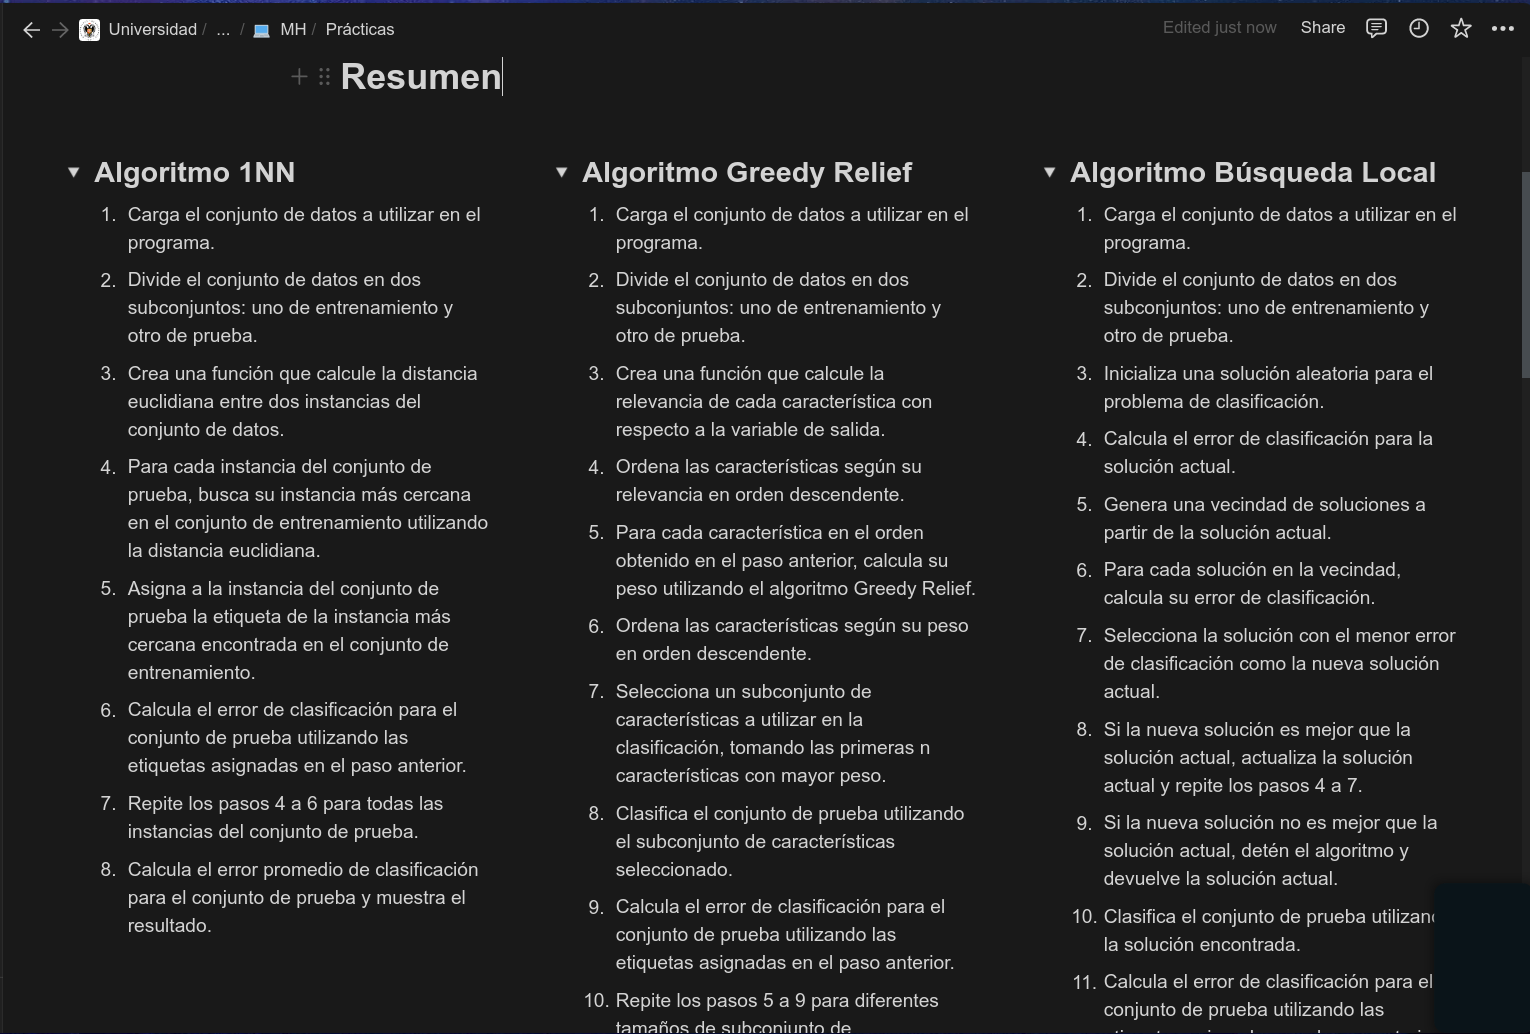
\includegraphics[width=\textwidth]{resumen.png}
		\caption{Estudio del problema}
		\label{fig:mi_imagen}
	\end{figure}

	\item Una vez se tiene claros los conceptos, creamos un nuevo directorio practicas1 con el material de prácticas. Creamos los directorios src, headers y reusamos el CMakeLists.txt y el random.hpp de tools.zip. Creamos un fichero .cpp y .h por algoritmo (esto cambiará) y el main.cpp. Los metemos en sus respectivos directorios y abrimos VScode.
	
	\item Primero vamos a definir una estructura de datos que será la base de todo el funcionamiento. En mi caso se abstraen los ejemplos en un Struct y se usa una clase Dataset para integrar vectores de ejemplos. Hardcodeamos una matriz de ejemplo y probamos hasta que funcione.
	
	\item Con la estructura montada pasamos a leer los datos. Para ello he recurrido a una practica de Estructura de Datos donde leía matrices de ficheros y la modifiqué para ignorar los comentarios y adaptarla al dataset.
	También he recurrido a Stackoverflow y chatgpt para las dudas. De paso configuramos el CMakeLists.txt con los ficheros de src y headers. IMPORTANTE: añadir optimización al compilador con el parámetro -02, será clave para la búsqueda local después.
	
	\item Llegados a este punto ya podemos empezar a implementar los métodos. Se implementarán en orden de dificultad y dependencia:
	\begin{enumerate}
		\item Algoritmo 1NN
		\item Algoritmo Greedy RELIEF
		\item Algoritmo Búsqueda Local Primer Mejor
		\item Algoritmo Genéticos: generacional y luego estacionario
		\item Algoritmos Meméticos: all, random y por último AM-best.
	\end{enumerate}
	Para verificar el correcto funcionamiento del algoritmo 1NN y la lectura de datos se ha recurrido a la  \href{https://mh2223.danimolina.net/testsol.html}{web de la asignatura} y junto a la ayuda de geeksforgeeks.org\cite{greekforgeeks}, una página muy recomendada para implementación de multitud algoritmos y problemas, se puede implementar el 1-NN sencillamente. 
	
	\item Una vez tenemos el clasificador pasamos a la implementación de Greedy y la BL. El pseudocódigo proporcionado de Greedy junto a la explicación del mismo en prácticas es suficiente para implementarlo aunque he consultado en la Universidad de Radboud \cite{runl} una tesis sobre la aplicación de algoritmos RELIEF en bioinformática. En cambio para la búsqueda Local, el pseudocódigo de teoría es insuficiente por lo que he recurrido nuevamente a Internet. Encontré un documento de la Universidad de la Laguna sobre sistemas Inteligentes \cite{ull}. En la página 43 encontramos un pseudocódigo más completo y del que nos basaremos para implementarlo. Para modular el código se ha utilizado los esquemas dados en el guión de prácticas.
	
	\item Para la implementación de los algoritmos genéticos podemos usar el repositorio de innovaMH \cite{innovaMH} proporcionado por Daniel Molina. Levantando docker localmente y observando la parte2.jl se entiende perfectamente y con gran detalle como implementar los algoritmos genéticos. 
	
	\item Para la implementación de los algoritmos meméticos he recurrido al seminario y guión que junto a los algoritmos genéticos ya implementados podemos completarlos sin dificultad.
\end{itemize}

\section{Experimentos}
El formato de ejecución de la práctica es:\\
\code{./practica1 <Algoritmo>  \  <Semilla(\textit{opcional})>}\\

Para los algoritmos GENÉTICOS se le añade como parámetro el operador:\\
\code{./practica1 <Algoritmo>  \  <Operador(\textit{BLX por defecto})> \ <Semilla(\textit{opcional})>}\\

Donde:
\begin{itemize}
	\item \code{<Algoritmo>} puede ser: 'sin parametro/vacio', 'oneNN', 'Greedy', 'BL', 'AGG', 'AGE', 'AM-All', 'AM-Rand', 'AM-Best'.
	
	\item \code{<Operador>} puede ser: 'sin parametro/vacio', 'Aritmetrico', 'BLX'.
	\item \code{<Semilla>} puede ser cualquier número.
\end{itemize}

Por ejemplo:
\begin{itemize}
	\item \code{./practica1 }: ejecutará la práctica con el clasificador 1-NN.
	\item \code{./practica1 AM-Rand}: ejecutará la práctica con el clasificador 1-NN mejorado con el Algoritmo Memético Aleatorio, operador BLX y semilla aleatoria.
	\item \code{./practica1 AGG Aritmetrico}: ejecutará la práctica con el clasificador 1-NN mejorado con el Algoritmo Genético Generacional, operador Aritmetrico y semilla aleatoria.
	\item \code{./practica1 AGE BLX 1}: ejecutará la práctica con el clasificador 1-NN mejorado con el Algoritmo Genético Estacionario, operador BLX y semilla 1.
\end{itemize}

\begin{figure}[h]
	\centering
	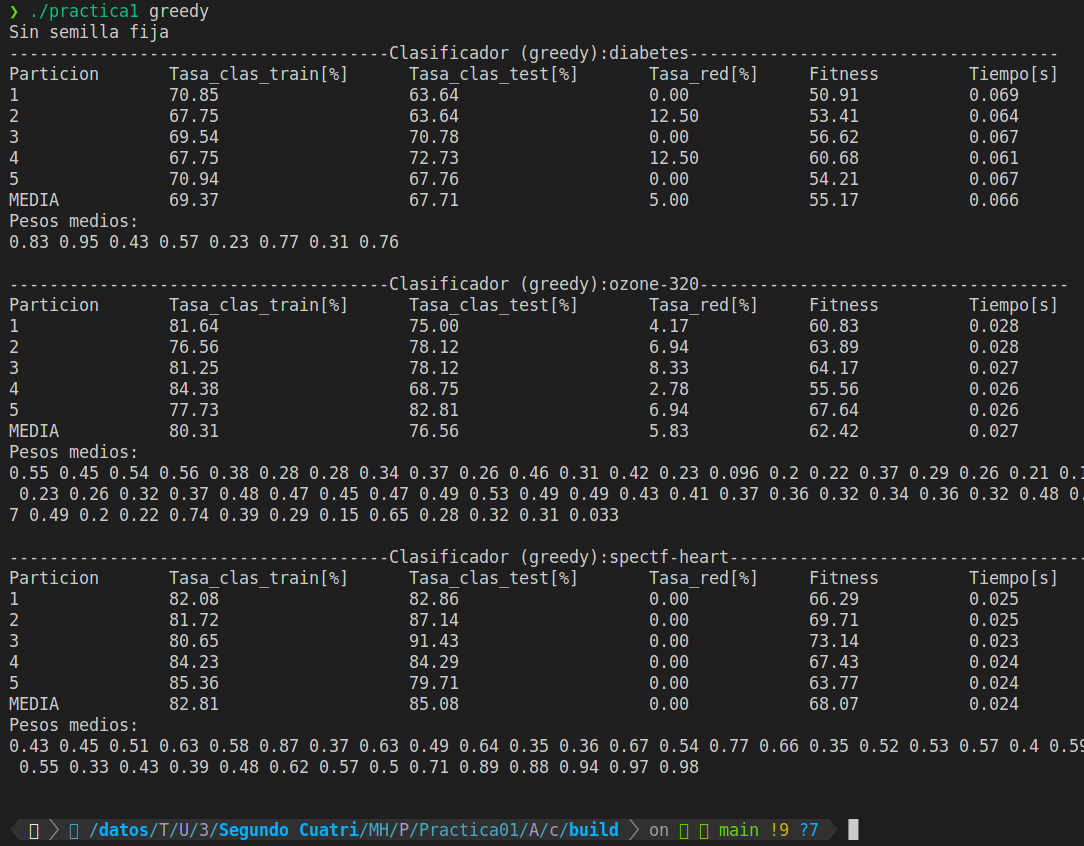
\includegraphics[width=\textwidth]{greedy.png}
	\caption{Ejecución de Greedy}
	\label{fig:greedy}
\end{figure}
Nota: Se añade la tasa\_clas de entrenamiento para comparar en la web. Se puede desactivar quitando el parámetro \code{true} en la linea 142 en main.cpp. Para la ejecución de las tablas siguientes se ha desactivado para mejorar los tiempos. \\

\subsection{Resultados algoritmos de búsqueda}
Las tablas que se presentan a continuación corresponden a resultados obtenidos por tres algoritmos (1NN, greedy y BL) aplicados al problema del Aprendizaje de Pesos en Características (APC) en tres conjuntos de datos diferentes (Diabetes, Ozone y Spectf-heart). Cada tabla muestra los porcentajes de clasificación, reducción del número de características, fitness y tiempo de ejecución para cada partición del conjunto de datos. Se busca comparar la eficacia de ambos algoritmos en términos de calidad de la solución y tiempo de ejecución.

% Please add the following required packages to your document preamble:
% \usepackage{multirow}
% \usepackage[table,xcdraw]{xcolor}
% If you use beamer only pass "xcolor=table" option, i.e. \documentclass[xcolor=table]{beamer}
\begin{table}[H]
	\caption{Resultados obtenidos por el clasificador 1NN en el problema del APC												
	}
	\label{tab:1nn}
	\resizebox{\textwidth}{!}{%
	\begin{tabular}{ccccccccccccc}
		\cline{2-13}
		&
		\multicolumn{4}{c}{\cellcolor[HTML]{C0C0C0}\textbf{Diabetes}} &
		\multicolumn{4}{c}{\cellcolor[HTML]{C0C0C0}\textbf{Ozone}} &
		\multicolumn{4}{c}{\cellcolor[HTML]{C0C0C0}\textbf{Spectf-heart}} \\ \cline{2-13} 
		\multirow{-2}{*}{} &
		\cellcolor[HTML]{DAE8FC}\textit{\textbf{\%\_clas}} &
		\cellcolor[HTML]{DAE8FC}\textit{\textbf{\%\_red}} &
		\cellcolor[HTML]{DAE8FC}\textit{\textbf{Fit.}} &
		\multicolumn{1}{c|}{\cellcolor[HTML]{DAE8FC}\textbf{T}} &
		\cellcolor[HTML]{DAE8FC}\textit{\textbf{\%\_clas}} &
		\cellcolor[HTML]{DAE8FC}\textit{\textbf{\%\_red}} &
		\cellcolor[HTML]{DAE8FC}\textit{\textbf{Fit.}} &
		\multicolumn{1}{c|}{\cellcolor[HTML]{DAE8FC}\textbf{T}} &
		\cellcolor[HTML]{DAE8FC}\textit{\textbf{\%\_clas}} &
		\cellcolor[HTML]{DAE8FC}\textit{\textbf{\%\_red}} &
		\cellcolor[HTML]{DAE8FC}\textit{\textbf{Fit.}} &
		\cellcolor[HTML]{DAE8FC}\textbf{T} \\ \cline{2-13} 
		\multicolumn{1}{c|}{\cellcolor[HTML]{C0C0C0}\textbf{1}} &
		\multicolumn{1}{c|}{66.88} &
		\multicolumn{1}{c|}{0.00} &
		\multicolumn{1}{c|}{53.51} &
		\multicolumn{1}{c|}{0.009} &
		\multicolumn{1}{c|}{78.12} &
		\multicolumn{1}{c|}{0.00} &
		\multicolumn{1}{c|}{62.50} &
		\multicolumn{1}{c|}{0.003} &
		\multicolumn{1}{c|}{77.14} &
		\multicolumn{1}{c|}{0.00} &
		\multicolumn{1}{c|}{61.71} &
		\multicolumn{1}{c|}{0.002} \\ \cline{2-13} 
		\multicolumn{1}{c|}{\cellcolor[HTML]{C0C0C0}\textbf{2}} &
		\multicolumn{1}{c|}{66.88} &
		\multicolumn{1}{c|}{0.00} &
		\multicolumn{1}{c|}{53.51} &
		\multicolumn{1}{c|}{0.009} &
		\multicolumn{1}{c|}{85.94} &
		\multicolumn{1}{c|}{0.00} &
		\multicolumn{1}{c|}{68.75} &
		\multicolumn{1}{c|}{0.003} &
		\multicolumn{1}{c|}{88.57} &
		\multicolumn{1}{c|}{0.00} &
		\multicolumn{1}{c|}{70.86} &
		\multicolumn{1}{c|}{0.003} \\ \cline{2-13} 
		\multicolumn{1}{c|}{\cellcolor[HTML]{C0C0C0}\textbf{3}} &
		\multicolumn{1}{c|}{68.83} &
		\multicolumn{1}{c|}{0.00} &
		\multicolumn{1}{c|}{55.06} &
		\multicolumn{1}{c|}{0.007} &
		\multicolumn{1}{c|}{79.69} &
		\multicolumn{1}{c|}{0.00} &
		\multicolumn{1}{c|}{63.75} &
		\multicolumn{1}{c|}{0.003} &
		\multicolumn{1}{c|}{91.43} &
		\multicolumn{1}{c|}{0.00} &
		\multicolumn{1}{c|}{73.14} &
		\multicolumn{1}{c|}{0.003} \\ \cline{2-13} 
		\multicolumn{1}{c|}{\cellcolor[HTML]{C0C0C0}\textbf{4}} &
		\multicolumn{1}{c|}{69.48} &
		\multicolumn{1}{c|}{0.00} &
		\multicolumn{1}{c|}{55.58} &
		\multicolumn{1}{c|}{0.008} &
		\multicolumn{1}{c|}{76.56} &
		\multicolumn{1}{c|}{0.00} &
		\multicolumn{1}{c|}{61.25} &
		\multicolumn{1}{c|}{0.003} &
		\multicolumn{1}{c|}{85.71} &
		\multicolumn{1}{c|}{0.00} &
		\multicolumn{1}{c|}{68.57} &
		\multicolumn{1}{c|}{0.002} \\ \cline{2-13} 
		\multicolumn{1}{c|}{\cellcolor[HTML]{C0C0C0}\textbf{5}} &
		\multicolumn{1}{c|}{69.74} &
		\multicolumn{1}{c|}{0.00} &
		\multicolumn{1}{c|}{55.79} &
		\multicolumn{1}{c|}{0.008} &
		\multicolumn{1}{c|}{81.25} &
		\multicolumn{1}{c|}{0.00} &
		\multicolumn{1}{c|}{65.00} &
		\multicolumn{1}{c|}{0.003} &
		\multicolumn{1}{c|}{84.06} &
		\multicolumn{1}{c|}{0.00} &
		\multicolumn{1}{c|}{67.25} &
		\multicolumn{1}{c|}{0.003} \\ \cline{2-13} 
		\multicolumn{1}{c|}{\cellcolor[HTML]{FFFE65}M} &
		\multicolumn{1}{c|}{\textbf{68.36}} &
		\multicolumn{1}{c|}{\textbf{0.00}} &
		\multicolumn{1}{c|}{\textbf{54.69}} &
		\multicolumn{1}{c|}{\textbf{0.0082}} &
		\multicolumn{1}{c|}{\textbf{80.31}} &
		\multicolumn{1}{c|}{\textbf{0.00}} &
		\multicolumn{1}{c|}{\textbf{64.25}} &
		\multicolumn{1}{c|}{\textbf{0.003}} &
		\multicolumn{1}{c|}{\textbf{85.38}} &
		\multicolumn{1}{c|}{\textbf{0.00}} &
		\multicolumn{1}{c|}{\textbf{68.31}} &
		\multicolumn{1}{c|}{\textbf{0.0026}} \\ \cline{2-13} 
	\end{tabular}
}
\end{table}

En la tabla \ref{tab:1nn} se puede observar que los resultados de clasificación son bastante buenos con un porcentaje de clasificación correcta de hasta el 85\% en spectf-heart. El porcentaje de reducción en el número de características es del 0\% ya que no se aplica ninguna selección de características.\\

Los valores de fitness oscilan entre 54,69 y 68,31, lo que indica que el algoritmo no ha encontrado necesariamente las soluciones óptimas para todos los conjuntos de datos. Por último, los tiempos de ejecución son bastante bajos, con valores inferiores a 0,01 segundos para todos los conjuntos de datos y particiones.

% Please add the following required packages to your document preamble:
% \usepackage{multirow}
% \usepackage[table,xcdraw]{xcolor}
% If you use beamer only pass "xcolor=table" option, i.e. \documentclass[xcolor=table]{beamer}
\begin{table}[H]
	\centering
	\caption{Resultados obtenidos por el algoritmo greedy en el problema del APC												
	}
	\label{tab:Greedy}
	\resizebox{\textwidth}{!}{%
	\begin{tabular}{ccccccccccccc}
		&
		\multicolumn{4}{c}{\cellcolor[HTML]{C0C0C0}\textbf{Diabetes}} &
		\multicolumn{4}{c}{\cellcolor[HTML]{C0C0C0}\textbf{Ozone}} &
		\multicolumn{4}{c}{\cellcolor[HTML]{C0C0C0}\textbf{Spectf-heart}} \\
		\multirow{-2}{*}{} &
		\cellcolor[HTML]{DAE8FC}\textit{\textbf{\%\_clas}} &
		\cellcolor[HTML]{DAE8FC}\textit{\textbf{\%\_red}} &
		\cellcolor[HTML]{DAE8FC}\textit{\textbf{Fit.}} &
		\cellcolor[HTML]{DAE8FC}\textbf{T} &
		\cellcolor[HTML]{DAE8FC}\textit{\textbf{\%\_clas}} &
		\cellcolor[HTML]{DAE8FC}\textit{\textbf{\%\_red}} &
		\cellcolor[HTML]{DAE8FC}\textit{\textbf{Fit.}} &
		\cellcolor[HTML]{DAE8FC}\textbf{T} &
		\cellcolor[HTML]{DAE8FC}\textit{\textbf{\%\_clas}} &
		\cellcolor[HTML]{DAE8FC}\textit{\textbf{\%\_red}} &
		\cellcolor[HTML]{DAE8FC}\textit{\textbf{Fit.}} &
		\cellcolor[HTML]{DAE8FC}\textbf{T} \\ \cline{2-13} 
		\multicolumn{1}{c|}{\cellcolor[HTML]{C0C0C0}\textbf{1}} &
		\multicolumn{1}{c|}{63.64} &
		\multicolumn{1}{c|}{0.00} &
		\multicolumn{1}{c|}{50.91} &
		\multicolumn{1}{c|}{0.034} &
		\multicolumn{1}{c|}{75.00} &
		\multicolumn{1}{c|}{4.17} &
		\multicolumn{1}{c|}{60.83} &
		\multicolumn{1}{c|}{0.031} &
		\multicolumn{1}{c|}{82.86} &
		\multicolumn{1}{c|}{0.00} &
		\multicolumn{1}{c|}{66.29} &
		\multicolumn{1}{c|}{0.026} \\ \cline{2-13} 
		\multicolumn{1}{c|}{\cellcolor[HTML]{C0C0C0}\textbf{2}} &
		\multicolumn{1}{c|}{63.64} &
		\multicolumn{1}{c|}{12.50} &
		\multicolumn{1}{c|}{53.41} &
		\multicolumn{1}{c|}{0.026} &
		\multicolumn{1}{c|}{78.12} &
		\multicolumn{1}{c|}{6.94} &
		\multicolumn{1}{c|}{63.89} &
		\multicolumn{1}{c|}{0.028} &
		\multicolumn{1}{c|}{87.14} &
		\multicolumn{1}{c|}{0.00} &
		\multicolumn{1}{c|}{69.71} &
		\multicolumn{1}{c|}{0.027} \\ \cline{2-13} 
		\multicolumn{1}{c|}{\cellcolor[HTML]{C0C0C0}\textbf{3}} &
		\multicolumn{1}{c|}{70.78} &
		\multicolumn{1}{c|}{0.00} &
		\multicolumn{1}{c|}{56.62} &
		\multicolumn{1}{c|}{0.023} &
		\multicolumn{1}{c|}{78.12} &
		\multicolumn{1}{c|}{8.33} &
		\multicolumn{1}{c|}{64.17} &
		\multicolumn{1}{c|}{0.029} &
		\multicolumn{1}{c|}{91.43} &
		\multicolumn{1}{c|}{0.00} &
		\multicolumn{1}{c|}{73.14} &
		\multicolumn{1}{c|}{0.024} \\ \cline{2-13} 
		\multicolumn{1}{c|}{\cellcolor[HTML]{C0C0C0}\textbf{4}} &
		\multicolumn{1}{c|}{72.73} &
		\multicolumn{1}{c|}{12.50} &
		\multicolumn{1}{c|}{60.68} &
		\multicolumn{1}{c|}{0.025} &
		\multicolumn{1}{c|}{68.75} &
		\multicolumn{1}{c|}{2.78} &
		\multicolumn{1}{c|}{55.56} &
		\multicolumn{1}{c|}{0.031} &
		\multicolumn{1}{c|}{84.29} &
		\multicolumn{1}{c|}{0.00} &
		\multicolumn{1}{c|}{67.43} &
		\multicolumn{1}{c|}{0.025} \\ \cline{2-13} 
		\multicolumn{1}{c|}{\cellcolor[HTML]{C0C0C0}\textbf{5}} &
		\multicolumn{1}{c|}{67.76} &
		\multicolumn{1}{c|}{0.00} &
		\multicolumn{1}{c|}{54.21} &
		\multicolumn{1}{c|}{0.031} &
		\multicolumn{1}{c|}{82.81} &
		\multicolumn{1}{c|}{6.94} &
		\multicolumn{1}{c|}{67.64} &
		\multicolumn{1}{c|}{0.03} &
		\multicolumn{1}{c|}{79.71} &
		\multicolumn{1}{c|}{0.00} &
		\multicolumn{1}{c|}{63.77} &
		\multicolumn{1}{c|}{0.027} \\ \cline{2-13} 
		\multicolumn{1}{c|}{\cellcolor[HTML]{FFFE65}M} &
		\multicolumn{1}{c|}{\textbf{67.71}} &
		\multicolumn{1}{c|}{\textbf{5.00}} &
		\multicolumn{1}{c|}{\textbf{55.17}} &
		\multicolumn{1}{c|}{\textbf{0.028}} &
		\multicolumn{1}{c|}{\textbf{76.56}} &
		\multicolumn{1}{c|}{\textbf{5.83}} &
		\multicolumn{1}{c|}{\textbf{62.42}} &
		\multicolumn{1}{c|}{\textbf{0.03}} &
		\multicolumn{1}{c|}{\textbf{85.08}} &
		\multicolumn{1}{c|}{\textbf{0.00}} &
		\multicolumn{1}{c|}{\textbf{68.07}} &
		\multicolumn{1}{c|}{\textbf{0.026}} \\ \cline{2-13} 
	\end{tabular}
}
\end{table}

En la tabla \ref{tab:Greedy} se observa que la media de los fitness obtenidos para cada conjunto de datos varía entre 55.17 y 68.07, lo que indica que el algoritmo es capaz de encontrar soluciones de igual calidad que el 1NN.\\

La diferencia está en que el \% de reducción en el número de características seleccionadas varía entre 0\% y 12.5\%, lo que significa que el algoritmo no siempre es capaz de reducir significativamente el número de características sin comprometer el rendimiento del modelo. Esto se debe a que Greedy maximiza la tasa\_clas, no el fitness al completo por lo que no tiende a reducir. Al igual que el 1NN, los tiempos son rápidos.

% Please add the following required packages to your document preamble:
% \usepackage{multirow}
% \usepackage[table,xcdraw]{xcolor}
% If you use beamer only pass "xcolor=table" option, i.e. \documentclass[xcolor=table]{beamer}
\begin{table}[H]
	\centering
	\caption{Resultados obtenidos por el algoritmo BL en el problema del APC												
	}
	\label{tab:bl}
	\resizebox{\textwidth}{!}{%
	\begin{tabular}{ccccccccccccc}
		\cline{2-13}
		&
		\multicolumn{4}{c}{\cellcolor[HTML]{C0C0C0}\textbf{Diabetes}} &
		\multicolumn{4}{c}{\cellcolor[HTML]{C0C0C0}\textbf{Ozone}} &
		\multicolumn{4}{c}{\cellcolor[HTML]{C0C0C0}\textbf{Spectf-heart}} \\ \cline{2-13} 
		\multirow{-2}{*}{} &
		\cellcolor[HTML]{DAE8FC}\textit{\textbf{\%\_clas}} &
		\cellcolor[HTML]{DAE8FC}\textit{\textbf{\%\_red}} &
		\cellcolor[HTML]{DAE8FC}\textit{\textbf{Fit.}} &
		\multicolumn{1}{c|}{\cellcolor[HTML]{DAE8FC}\textbf{T}} &
		\cellcolor[HTML]{DAE8FC}\textit{\textbf{\%\_clas}} &
		\cellcolor[HTML]{DAE8FC}\textit{\textbf{\%\_red}} &
		\cellcolor[HTML]{DAE8FC}\textit{\textbf{Fit.}} &
		\multicolumn{1}{c|}{\cellcolor[HTML]{DAE8FC}\textbf{T}} &
		\cellcolor[HTML]{DAE8FC}\textit{\textbf{\%\_clas}} &
		\cellcolor[HTML]{DAE8FC}\textit{\textbf{\%\_red}} &
		\cellcolor[HTML]{DAE8FC}\textit{\textbf{Fit.}} &
		\cellcolor[HTML]{DAE8FC}\textbf{T} \\ \cline{2-13} 
		\multicolumn{1}{c|}{\cellcolor[HTML]{C0C0C0}\textbf{1}} &
		\multicolumn{1}{c|}{70.78} &
		\multicolumn{1}{c|}{62.50} &
		\multicolumn{1}{c|}{69.12} &
		\multicolumn{1}{c|}{6.4} &
		\multicolumn{1}{c|}{76.56} &
		\multicolumn{1}{c|}{15.28} &
		\multicolumn{1}{c|}{64.31} &
		\multicolumn{1}{c|}{22} &
		\multicolumn{1}{c|}{72.86} &
		\multicolumn{1}{c|}{52.27} &
		\multicolumn{1}{c|}{68.74} &
		\multicolumn{1}{c|}{15} \\ \cline{2-13} 
		\multicolumn{1}{c|}{\cellcolor[HTML]{C0C0C0}\textbf{2}} &
		\multicolumn{1}{c|}{72.08} &
		\multicolumn{1}{c|}{62.50} &
		\multicolumn{1}{c|}{70.16} &
		\multicolumn{1}{c|}{13} &
		\multicolumn{1}{c|}{84.38} &
		\multicolumn{1}{c|}{48.61} &
		\multicolumn{1}{c|}{77.22} &
		\multicolumn{1}{c|}{47} &
		\multicolumn{1}{c|}{85.71} &
		\multicolumn{1}{c|}{45.45} &
		\multicolumn{1}{c|}{77.66} &
		\multicolumn{1}{c|}{16} \\ \cline{2-13} 
		\multicolumn{1}{c|}{\cellcolor[HTML]{C0C0C0}\textbf{3}} &
		\multicolumn{1}{c|}{68.18} &
		\multicolumn{1}{c|}{75.00} &
		\multicolumn{1}{c|}{69.55} &
		\multicolumn{1}{c|}{18} &
		\multicolumn{1}{c|}{78.12} &
		\multicolumn{1}{c|}{43.06} &
		\multicolumn{1}{c|}{71.11} &
		\multicolumn{1}{c|}{37} &
		\multicolumn{1}{c|}{90.00} &
		\multicolumn{1}{c|}{34.09} &
		\multicolumn{1}{c|}{78.82} &
		\multicolumn{1}{c|}{11} \\ \cline{2-13} 
		\multicolumn{1}{c|}{\cellcolor[HTML]{C0C0C0}\textbf{4}} &
		\multicolumn{1}{c|}{63.64} &
		\multicolumn{1}{c|}{75.00} &
		\multicolumn{1}{c|}{65.91} &
		\multicolumn{1}{c|}{15} &
		\multicolumn{1}{c|}{70.31} &
		\multicolumn{1}{c|}{43.06} &
		\multicolumn{1}{c|}{64.86} &
		\multicolumn{1}{c|}{24} &
		\multicolumn{1}{c|}{82.86} &
		\multicolumn{1}{c|}{70.45} &
		\multicolumn{1}{c|}{80.38} &
		\multicolumn{1}{c|}{18} \\ \cline{2-13} 
		\multicolumn{1}{c|}{\cellcolor[HTML]{C0C0C0}\textbf{5}} &
		\multicolumn{1}{c|}{71.71} &
		\multicolumn{1}{c|}{75.00} &
		\multicolumn{1}{c|}{72.37} &
		\multicolumn{1}{c|}{6.1} &
		\multicolumn{1}{c|}{82.81} &
		\multicolumn{1}{c|}{47.22} &
		\multicolumn{1}{c|}{75.69} &
		\multicolumn{1}{c|}{30} &
		\multicolumn{1}{c|}{81.16} &
		\multicolumn{1}{c|}{59.09} &
		\multicolumn{1}{c|}{76.75} &
		\multicolumn{1}{c|}{15} \\ \cline{2-13} 
		\multicolumn{1}{c|}{\cellcolor[HTML]{FFFE65}\textbf{M}} &
		\multicolumn{1}{c|}{\textbf{69.28}} &
		\multicolumn{1}{c|}{\textbf{70.00}} &
		\multicolumn{1}{c|}{\textbf{69.42}} &
		\multicolumn{1}{c|}{\textbf{12}} &
		\multicolumn{1}{c|}{\textbf{78.44}} &
		\multicolumn{1}{c|}{\textbf{39.44}} &
		\multicolumn{1}{c|}{\textbf{70.64}} &
		\multicolumn{1}{c|}{\textbf{32}} &
		\multicolumn{1}{c|}{\textbf{82.52}} &
		\multicolumn{1}{c|}{\textbf{52.27}} &
		\multicolumn{1}{c|}{\textbf{76.47}} &
		\multicolumn{1}{c|}{\textbf{15}} \\ \cline{2-13} 
	\end{tabular}
}
\end{table}
Al analizar los resultados de la tabla \ref{tab:bl}, se observa que el algoritmo BL obtiene mejores resultados que el algoritmo Greedy y 1-NN en términos de fitness para todas las particiones y conjuntos de datos. Además, el porcentaje de reducción es significativamente mayor en promedio para el algoritmo BL, lo que sugiere que el número de características seleccionadas es menor en comparación con el algoritmo Greedy.\\

Sin embargo, podemos observar el alto coste computacional que supone ejecutar la búsqueda. Los tiempos multiplican por cientos al de Greedy y 1NN.

% Please add the following required packages to your document preamble:
% \usepackage{graphicx}
% \usepackage[table,xcdraw]{xcolor}
% If you use beamer only pass "xcolor=table" option, i.e. \documentclass[xcolor=table]{beamer}
\begin{table}[H]
	\centering
	\caption{Resultados obtenidos por la BMB y los algoritmos de Trayectoria en el problema del APC}
	\label{tab:final}
	\resizebox{\textwidth}{!}{%
		\begin{tabular}{c|cccc|cccc|cccc|}
			\cline{2-13}
			\multicolumn{1}{l|}{\textbf{}} &
			\multicolumn{4}{c|}{\textbf{Diabetes}} &
			\multicolumn{4}{c|}{\textbf{Ozone}} &
			\multicolumn{4}{c|}{\textbf{Spectf-heart}} \\ \cline{2-13} 
			\multicolumn{1}{l|}{\textbf{}} &
			\multicolumn{1}{c|}{\textbf{\%\_clas}} &
			\multicolumn{1}{c|}{\textbf{\%\_red}} &
			\multicolumn{1}{c|}{\textbf{Fit.}} &
			\textbf{T{[}s{]}} &
			\multicolumn{1}{c|}{\textbf{\%\_clas}} &
			\multicolumn{1}{c|}{\textbf{\%\_red}} &
			\multicolumn{1}{c|}{\textbf{Fit.}} &
			\textbf{T{[}s{]}} &
			\multicolumn{1}{c|}{\textbf{\%\_clas}} &
			\multicolumn{1}{c|}{\textbf{\%\_red}} &
			\multicolumn{1}{c|}{\textbf{Fit.}} &
			\textbf{T{[}s{]}} \\ \hline
			\multicolumn{1}{|c|}{\textbf{BL}} &
			\multicolumn{1}{c|}{69.66} &
			\multicolumn{1}{c|}{62.50} &
			\multicolumn{1}{c|}{68.23} &
			1.8 &
			\multicolumn{1}{c|}{79.69} &
			\multicolumn{1}{c|}{37.78} &
			\multicolumn{1}{c|}{71.31} &
			16 &
			\multicolumn{1}{c|}{84.51} &
			\multicolumn{1}{c|}{48.18} &
			\multicolumn{1}{c|}{77.25} &
			6.3 \\ \hline
			\multicolumn{1}{|c|}{\textbf{BMB}} &
			\multicolumn{1}{c|}{67.19} &
			\multicolumn{1}{c|}{67.50} &
			\multicolumn{1}{c|}{67.26} &
			22 &
			\multicolumn{1}{c|}{78.44} &
			\multicolumn{1}{c|}{46.67} &
			\multicolumn{1}{c|}{72.08} &
			72 &
			\multicolumn{1}{c|}{84.82} &
			\multicolumn{1}{c|}{62.73} &
			\multicolumn{1}{c|}{80.40} &
			56 \\ \hline
			\multicolumn{1}{|c|}{\textbf{ES}} &
			\multicolumn{1}{c|}{68.49} &
			\multicolumn{1}{c|}{65.00} &
			\multicolumn{1}{c|}{67.79} &
			69 &
			\multicolumn{1}{c|}{77.81} &
			\multicolumn{1}{c|}{58.33} &
			\multicolumn{1}{c|}{73.92} &
			82 &
			\multicolumn{1}{c|}{83.93} &
			\multicolumn{1}{c|}{60.45} &
			\multicolumn{1}{c|}{79.24} &
			58 \\ \hline
			\multicolumn{1}{|c|}{\textbf{ILS}} &
			\multicolumn{1}{c|}{68.36} &
			\multicolumn{1}{c|}{67.50} &
			\multicolumn{1}{c|}{68.19} &
			20 &
			\multicolumn{1}{c|}{80.94} &
			\multicolumn{1}{c|}{51.94} &
			\multicolumn{1}{c|}{75.14} &
			89 &
			\multicolumn{1}{c|}{83.95} &
			\multicolumn{1}{c|}{66.36} &
			\multicolumn{1}{c|}{80.43} &
			58 \\ \hline
			\multicolumn{1}{|c|}{{\color[HTML]{FE0000} \textbf{ILS-ES}}} &
			\multicolumn{1}{c|}{66.29} &
			\multicolumn{1}{c|}{75.00} &
			\multicolumn{1}{c|}{68.03} &
			71 &
			\multicolumn{1}{c|}{81.56} &
			\multicolumn{1}{c|}{56.11} &
			\multicolumn{1}{c|}{{\color[HTML]{00009B} \textbf{76.47}}} &
			94 &
			\multicolumn{1}{c|}{85.95} &
			\multicolumn{1}{c|}{69.55} &
			\multicolumn{1}{c|}{{\color[HTML]{00009B} \textbf{82.67}}} &
			68 \\ \hline
			\multicolumn{1}{|c|}{\textbf{VNS}} &
			\multicolumn{1}{c|}{66.54} &
			\multicolumn{1}{c|}{75.00} &
			\multicolumn{1}{c|}{{\color[HTML]{00009B} \textbf{68.24}}} &
			23 &
			\multicolumn{1}{c|}{78.75} &
			\multicolumn{1}{c|}{45.00} &
			\multicolumn{1}{c|}{72.00} &
			87 &
			\multicolumn{1}{c|}{85.38} &
			\multicolumn{1}{c|}{51.36} &
			\multicolumn{1}{c|}{78.58} &
			56 \\ \hline
		\end{tabular}%
	}
\end{table}

En la tabla \ref{tab:final} se presentan los resultados globales para los tres algoritmos en los tres conjuntos de datos. En general, el \textbf{algoritmo BL} tuvo un mejor rendimiento en términos de porcentaje de reducción y agregación, aunque tuvo una reducción de dimensiones más alta. El algoritmo 1-NN es el mejor en términos de porcentaje de clasificación, pero no es capaz de reducir la dimensionalidad del conjunto de datos. Por otro lado, el algoritmo RELIEF tuvo un desempeño inferior en comparación con BL, aunque logró reducir algo la dimensionalidad del conjunto de datos.\\

En cuanto a los conjuntos de datos individuales, en Diabetes, los tres algoritmos lograron un rendimiento similar en términos de porcentaje de clasificación y agregación, aunque BL tuvo la reducción de dimensionalidad más alta. En Ozone, BL tuvo un mejor rendimiento que 1-NN y RELIEF en términos de porcentaje de clasificación y agregación, pero también tuvo una reducción de dimensionalidad más alta. En Spectf-heart, BL también tuvo un mejor rendimiento en comparación con 1-NN y RELIEF, aunque tuvo una reducción de dimensionalidad más alta.\\

\subsection{Resultados Algoritmos Genéticos y Meméticos}

% Please add the following required packages to your document preamble:
% \usepackage{graphicx}
% \usepackage[table,xcdraw]{xcolor}
% If you use beamer only pass "xcolor=table" option, i.e. \documentclass[xcolor=table]{beamer}
\begin{table}[H]
	\centering
	\caption{Resultados obtenidos por el algoritmo AGG-CA en el problema del APC}
	\label{tab:AGG_CA}
	\resizebox{\textwidth}{!}{%
		\begin{tabular}{ccccccccccccc}
			\rowcolor[HTML]{D9D9D9} 
			\multicolumn{1}{l}{\cellcolor[HTML]{FFFFFF}\textbf{}} &
			\multicolumn{4}{c}{\cellcolor[HTML]{D9D9D9}\textbf{Diabetes}} &
			\multicolumn{4}{c}{\cellcolor[HTML]{D9D9D9}\textbf{Ozone}} &
			\multicolumn{4}{c}{\cellcolor[HTML]{D9D9D9}\textbf{Spectf-heart}} \\
			\rowcolor[HTML]{CFE2F3} 
			\multicolumn{1}{l}{\cellcolor[HTML]{FFFFFF}\textbf{}} &
			\textbf{\%\_class} &
			\textbf{\%\_red} &
			\textbf{Fit.} &
			\textbf{T[s]} &
			\textbf{\%\_class} &
			\textbf{\%\_red} &
			\textbf{Fit.} &
			\textbf{T[s]} &
			\textbf{\%\_class} &
			\textbf{\%\_red} &
			\textbf{Fit.} &
			\textbf{T[s]} \\ \cline{2-13} 
			\multicolumn{1}{c|}{\cellcolor[HTML]{D9D9D9}\textbf{1}} &
			\multicolumn{1}{c|}{68.83} &
			\multicolumn{1}{c|}{50.00} &
			\multicolumn{1}{c|}{65.06} &
			\multicolumn{1}{c|}{68} &
			\multicolumn{1}{c|}{81.25} &
			\multicolumn{1}{c|}{25.00} &
			\multicolumn{1}{c|}{70.00} &
			\multicolumn{1}{c|}{70} &
			\multicolumn{1}{c|}{85.71} &
			\multicolumn{1}{c|}{29.55} &
			\multicolumn{1}{c|}{74.48} &
			\multicolumn{1}{c|}{51} \\ \cline{2-13} 
			\multicolumn{1}{c|}{\cellcolor[HTML]{D9D9D9}\textbf{2}} &
			\multicolumn{1}{c|}{68.18} &
			\multicolumn{1}{c|}{37.50} &
			\multicolumn{1}{c|}{62.05} &
			\multicolumn{1}{c|}{69} &
			\multicolumn{1}{c|}{76.56} &
			\multicolumn{1}{c|}{38.89} &
			\multicolumn{1}{c|}{69.03} &
			\multicolumn{1}{c|}{71} &
			\multicolumn{1}{c|}{87.14} &
			\multicolumn{1}{c|}{36.36} &
			\multicolumn{1}{c|}{76.99} &
			\multicolumn{1}{c|}{51} \\ \cline{2-13} 
			\multicolumn{1}{c|}{\cellcolor[HTML]{D9D9D9}\textbf{3}} &
			\multicolumn{1}{c|}{60.39} &
			\multicolumn{1}{c|}{75.00} &
			\multicolumn{1}{c|}{63.31} &
			\multicolumn{1}{c|}{65} &
			\multicolumn{1}{c|}{82.81} &
			\multicolumn{1}{c|}{33.33} &
			\multicolumn{1}{c|}{72.92} &
			\multicolumn{1}{c|}{70} &
			\multicolumn{1}{c|}{95.71} &
			\multicolumn{1}{c|}{22.73} &
			\multicolumn{1}{c|}{81.12} &
			\multicolumn{1}{c|}{49} \\ \cline{2-13} 
			\multicolumn{1}{c|}{\cellcolor[HTML]{D9D9D9}\textbf{4}} &
			\multicolumn{1}{c|}{66.23} &
			\multicolumn{1}{c|}{62.50} &
			\multicolumn{1}{c|}{65.49} &
			\multicolumn{1}{c|}{68} &
			\multicolumn{1}{c|}{71.88} &
			\multicolumn{1}{c|}{30.56} &
			\multicolumn{1}{c|}{63.61} &
			\multicolumn{1}{c|}{67} &
			\multicolumn{1}{c|}{78.57} &
			\multicolumn{1}{c|}{27.27} &
			\multicolumn{1}{c|}{68.31} &
			\multicolumn{1}{c|}{55} \\ \cline{2-13} 
			\multicolumn{1}{c|}{\cellcolor[HTML]{D9D9D9}\textbf{5}} &
			\multicolumn{1}{c|}{67.76} &
			\multicolumn{1}{c|}{37.50} &
			\multicolumn{1}{c|}{61.71} &
			\multicolumn{1}{c|}{70} &
			\multicolumn{1}{c|}{76.56} &
			\multicolumn{1}{c|}{20.83} &
			\multicolumn{1}{c|}{65.42} &
			\multicolumn{1}{c|}{74} &
			\multicolumn{1}{c|}{81.16} &
			\multicolumn{1}{c|}{36.36} &
			\multicolumn{1}{c|}{72.20} &
			\multicolumn{1}{c|}{53} \\ \cline{2-13} 
			\multicolumn{1}{c|}{\cellcolor[HTML]{FFFF00}\textbf{M}} &
			\multicolumn{1}{c|}{\textbf{66.28}} &
			\multicolumn{1}{c|}{\textbf{52.50}} &
			\multicolumn{1}{c|}{\textbf{63.52}} &
			\multicolumn{1}{c|}{\textbf{68}} &
			\multicolumn{1}{c|}{\textbf{77.81}} &
			\multicolumn{1}{c|}{\textbf{29.72}} &
			\multicolumn{1}{c|}{\textbf{68.19}} &
			\multicolumn{1}{c|}{\textbf{70}} &
			\multicolumn{1}{c|}{\textbf{85.66}} &
			\multicolumn{1}{c|}{\textbf{30.45}} &
			\multicolumn{1}{c|}{\textbf{74.62}} &
			\multicolumn{1}{c|}{\textbf{52}} \\ \cline{2-13} 
		\end{tabular}%
	}
\end{table}
En la tabla \ref{tab:AGG_CA} se puede observar que los resultados de clasificación son bastante buenos con un porcentaje de clasificación correcta de hasta el 85\% en spectf-heart. El porcentaje de reducción en el número de características es del 45\% aproximadamente aunque en diabetes reduce mucho mientras que el resto se queda en 30\%.\\

Los valores de fitness oscilan entre 63,52 y 74,62, lo que indica que el algoritmo no ha encontrado necesariamente las soluciones óptimas para todos los conjuntos de datos. Por último, los tiempos de ejecución son considerablemente altos en comparación a los algoritmos previos, de unos 50 segundos por partición.

% Please add the following required packages to your document preamble:
% \usepackage{graphicx}
% \usepackage[table,xcdraw]{xcolor}
% If you use beamer only pass "xcolor=table" option, i.e. \documentclass[xcolor=table]{beamer}
\begin{table}[H]
	\centering
	\caption{Resultados obtenidos por el algoritmo AGG-BLX en el problema del APC}
	\label{tab:AGG_BLX}
	\resizebox{\textwidth}{!}{%
		\begin{tabular}{ccccccccccccc}
			\rowcolor[HTML]{D9D9D9} 
			\multicolumn{1}{l}{\cellcolor[HTML]{FFFFFF}\textbf{}} &
			\multicolumn{4}{c}{\cellcolor[HTML]{D9D9D9}\textbf{Diabetes}} &
			\multicolumn{4}{c}{\cellcolor[HTML]{D9D9D9}\textbf{Ozone}} &
			\multicolumn{4}{c}{\cellcolor[HTML]{D9D9D9}\textbf{Spectf-heart}} \\
			\rowcolor[HTML]{CFE2F3} 
			\multicolumn{1}{l}{\cellcolor[HTML]{FFFFFF}\textbf{}} &
			\textbf{\%\_clas} &
			\textbf{\%\_red} &
			\textbf{Fit.} &
			\textbf{T[s]} &
			\textbf{\%\_clas} &
			\textbf{\%\_red} &
			\textbf{Fit.} &
			\textbf{T[s]} &
			\textbf{\%\_clas} &
			\textbf{\%\_red} &
			\textbf{Fit.} &
			\textbf{T[s]} \\ \cline{2-13} 
			\multicolumn{1}{c|}{\cellcolor[HTML]{D9D9D9}\textbf{1}} &
			\multicolumn{1}{c|}{72.08} &
			\multicolumn{1}{c|}{50.00} &
			\multicolumn{1}{c|}{67.66} &
			\multicolumn{1}{c|}{68} &
			\multicolumn{1}{c|}{76.56} &
			\multicolumn{1}{c|}{37.50} &
			\multicolumn{1}{c|}{68.75} &
			\multicolumn{1}{c|}{78} &
			\multicolumn{1}{c|}{81.43} &
			\multicolumn{1}{c|}{47.73} &
			\multicolumn{1}{c|}{74.69} &
			\multicolumn{1}{c|}{54} \\ \cline{2-13} 
			\multicolumn{1}{c|}{\cellcolor[HTML]{D9D9D9}\textbf{2}} &
			\multicolumn{1}{c|}{73.38} &
			\multicolumn{1}{c|}{50.00} &
			\multicolumn{1}{c|}{68.70} &
			\multicolumn{1}{c|}{68} &
			\multicolumn{1}{c|}{84.38} &
			\multicolumn{1}{c|}{36.11} &
			\multicolumn{1}{c|}{74.72} &
			\multicolumn{1}{c|}{79} &
			\multicolumn{1}{c|}{82.86} &
			\multicolumn{1}{c|}{38.64} &
			\multicolumn{1}{c|}{74.01} &
			\multicolumn{1}{c|}{55} \\ \cline{2-13} 
			\multicolumn{1}{c|}{\cellcolor[HTML]{D9D9D9}\textbf{3}} &
			\multicolumn{1}{c|}{63.64} &
			\multicolumn{1}{c|}{50.00} &
			\multicolumn{1}{c|}{60.91} &
			\multicolumn{1}{c|}{67} &
			\multicolumn{1}{c|}{76.56} &
			\multicolumn{1}{c|}{41.67} &
			\multicolumn{1}{c|}{69.58} &
			\multicolumn{1}{c|}{83} &
			\multicolumn{1}{c|}{91.43} &
			\multicolumn{1}{c|}{40.91} &
			\multicolumn{1}{c|}{81.32} &
			\multicolumn{1}{c|}{55} \\ \cline{2-13} 
			\multicolumn{1}{c|}{\cellcolor[HTML]{D9D9D9}\textbf{4}} &
			\multicolumn{1}{c|}{48.70} &
			\multicolumn{1}{c|}{87.50} &
			\multicolumn{1}{c|}{56.46} &
			\multicolumn{1}{c|}{67} &
			\multicolumn{1}{c|}{73.44} &
			\multicolumn{1}{c|}{34.72} &
			\multicolumn{1}{c|}{65.69} &
			\multicolumn{1}{c|}{78} &
			\multicolumn{1}{c|}{81.43} &
			\multicolumn{1}{c|}{36.36} &
			\multicolumn{1}{c|}{72.42} &
			\multicolumn{1}{c|}{56} \\ \cline{2-13} 
			\multicolumn{1}{c|}{\cellcolor[HTML]{D9D9D9}\textbf{5}} &
			\multicolumn{1}{c|}{58.55} &
			\multicolumn{1}{c|}{87.50} &
			\multicolumn{1}{c|}{64.34} &
			\multicolumn{1}{c|}{68} &
			\multicolumn{1}{c|}{84.38} &
			\multicolumn{1}{c|}{33.33} &
			\multicolumn{1}{c|}{74.17} &
			\multicolumn{1}{c|}{76} &
			\multicolumn{1}{c|}{76.81} &
			\multicolumn{1}{c|}{36.36} &
			\multicolumn{1}{c|}{68.72} &
			\multicolumn{1}{c|}{54} \\ \cline{2-13} 
			\multicolumn{1}{c|}{\cellcolor[HTML]{FFFF00}\textbf{M}} &
			\multicolumn{1}{c|}{\textbf{63.27}} &
			\multicolumn{1}{c|}{\textbf{65.00}} &
			\multicolumn{1}{c|}{\textbf{63.62}} &
			\multicolumn{1}{c|}{\textbf{68}} &
			\multicolumn{1}{c|}{\textbf{79.06}} &
			\multicolumn{1}{c|}{\textbf{36.67}} &
			\multicolumn{1}{c|}{\textbf{70.58}} &
			\multicolumn{1}{c|}{\textbf{79}} &
			\multicolumn{1}{c|}{\textbf{82.79}} &
			\multicolumn{1}{c|}{\textbf{40.00}} &
			\multicolumn{1}{c|}{\textbf{74.23}} &
			\multicolumn{1}{c|}{\textbf{55}} \\ \cline{2-13} 
		\end{tabular}%
	}
\end{table}
En la tabla \ref{tab:AGG_BLX} se puede observar que los resultados de clasificación han bajado respecto antes pero ha aumentado la reducción sensiblemente. El porcentaje de reducción en el número de características es del 50\% aproximadamente aunque en diabetes reduce mucho mientras que el resto se queda en 40\%.\\

Los valores de fitness oscilan entre 63,62 y 74,23, lo que indica que el operador de cruce no ha mejorado prácticamente EN MI CASO aunque debería ser algo mejor que el Aritmétrico aleatorio. Por último, los tiempos de ejecución son similares al anterior.

% Please add the following required packages to your document preamble:
% \usepackage{graphicx}
% \usepackage[table,xcdraw]{xcolor}
% If you use beamer only pass "xcolor=table" option, i.e. \documentclass[xcolor=table]{beamer}
\begin{table}[H]
	\centering
	\caption{Resultados obtenidos por el algoritmo AGE-CA en el problema del APC}
	\label{tab:AGE_CA}
	\resizebox{\textwidth}{!}{%
		\begin{tabular}{ccccccccccccc}
			\rowcolor[HTML]{D9D9D9} 
			\multicolumn{1}{l}{\cellcolor[HTML]{FFFFFF}\textbf{}} &
			\multicolumn{4}{c}{\cellcolor[HTML]{D9D9D9}\textbf{Diabetes}} &
			\multicolumn{4}{c}{\cellcolor[HTML]{D9D9D9}\textbf{Ozone}} &
			\multicolumn{4}{c}{\cellcolor[HTML]{D9D9D9}\textbf{Spectf-heart}} \\
			\rowcolor[HTML]{CFE2F3} 
			\multicolumn{1}{l}{\cellcolor[HTML]{FFFFFF}\textbf{}} &
			\textbf{\%\_clas} &
			\textbf{\%\_red} &
			\textbf{Fit.} &
			\textbf{T[s]} &
			\textbf{\%\_clas} &
			\textbf{\%\_red} &
			\textbf{Fit.} &
			\textbf{T[s]} &
			\textbf{\%\_clas} &
			\textbf{\%\_red} &
			\textbf{Fit.} &
			\textbf{T[s]} \\ \cline{2-13} 
			\multicolumn{1}{c|}{\cellcolor[HTML]{D9D9D9}\textbf{1}} &
			\multicolumn{1}{c|}{68.18} &
			\multicolumn{1}{c|}{62.50} &
			\multicolumn{1}{c|}{67.05} &
			\multicolumn{1}{c|}{80} &
			\multicolumn{1}{c|}{79.69} &
			\multicolumn{1}{c|}{16.67} &
			\multicolumn{1}{c|}{67.08} &
			\multicolumn{1}{c|}{96} &
			\multicolumn{1}{c|}{82.86} &
			\multicolumn{1}{c|}{20.45} &
			\multicolumn{1}{c|}{70.38} &
			\multicolumn{1}{c|}{77} \\ \cline{2-13} 
			\multicolumn{1}{c|}{\cellcolor[HTML]{D9D9D9}\textbf{2}} &
			\multicolumn{1}{c|}{64.94} &
			\multicolumn{1}{c|}{62.50} &
			\multicolumn{1}{c|}{64.45} &
			\multicolumn{1}{c|}{73} &
			\multicolumn{1}{c|}{79.69} &
			\multicolumn{1}{c|}{19.44} &
			\multicolumn{1}{c|}{67.64} &
			\multicolumn{1}{c|}{82} &
			\multicolumn{1}{c|}{88.57} &
			\multicolumn{1}{c|}{22.73} &
			\multicolumn{1}{c|}{75.40} &
			\multicolumn{1}{c|}{73} \\ \cline{2-13} 
			\multicolumn{1}{c|}{\cellcolor[HTML]{D9D9D9}\textbf{3}} &
			\multicolumn{1}{c|}{70.13} &
			\multicolumn{1}{c|}{62.50} &
			\multicolumn{1}{c|}{68.60} &
			\multicolumn{1}{c|}{82} &
			\multicolumn{1}{c|}{85.94} &
			\multicolumn{1}{c|}{13.89} &
			\multicolumn{1}{c|}{71.53} &
			\multicolumn{1}{c|}{73} &
			\multicolumn{1}{c|}{91.43} &
			\multicolumn{1}{c|}{18.18} &
			\multicolumn{1}{c|}{76.78} &
			\multicolumn{1}{c|}{75} \\ \cline{2-13} 
			\multicolumn{1}{c|}{\cellcolor[HTML]{D9D9D9}\textbf{4}} &
			\multicolumn{1}{c|}{68.18} &
			\multicolumn{1}{c|}{62.50} &
			\multicolumn{1}{c|}{67.05} &
			\multicolumn{1}{c|}{99} &
			\multicolumn{1}{c|}{71.88} &
			\multicolumn{1}{c|}{26.39} &
			\multicolumn{1}{c|}{62.78} &
			\multicolumn{1}{c|}{78} &
			\multicolumn{1}{c|}{81.43} &
			\multicolumn{1}{c|}{18.18} &
			\multicolumn{1}{c|}{68.78} &
			\multicolumn{1}{c|}{72} \\ \cline{2-13} 
			\multicolumn{1}{c|}{\cellcolor[HTML]{D9D9D9}\textbf{5}} &
			\multicolumn{1}{c|}{71.05} &
			\multicolumn{1}{c|}{50.00} &
			\multicolumn{1}{c|}{66.84} &
			\multicolumn{1}{c|}{99} &
			\multicolumn{1}{c|}{76.56} &
			\multicolumn{1}{c|}{16.67} &
			\multicolumn{1}{c|}{64.58} &
			\multicolumn{1}{c|}{92} &
			\multicolumn{1}{c|}{78.26} &
			\multicolumn{1}{c|}{31.82} &
			\multicolumn{1}{c|}{68.97} &
			\multicolumn{1}{c|}{54} \\ \cline{2-13} 
			\multicolumn{1}{c|}{\cellcolor[HTML]{FFFF00}\textbf{M}} &
			\multicolumn{1}{c|}{\textbf{68.50}} &
			\multicolumn{1}{c|}{\textbf{60.00}} &
			\multicolumn{1}{c|}{\textbf{66.80}} &
			\multicolumn{1}{c|}{\textbf{89}} &
			\multicolumn{1}{c|}{\textbf{78.75}} &
			\multicolumn{1}{c|}{\textbf{18.61}} &
			\multicolumn{1}{c|}{\textbf{66.72}} &
			\multicolumn{1}{c|}{\textbf{84}} &
			\multicolumn{1}{c|}{\textbf{84.51}} &
			\multicolumn{1}{c|}{\textbf{22.27}} &
			\multicolumn{1}{c|}{\textbf{72.06}} &
			\multicolumn{1}{c|}{\textbf{70}} \\ \cline{2-13} 
		\end{tabular}%
	}
\end{table}
En la tabla \ref{tab:AGE_CA} se puede observar que los resultados de clasificación vuelven a ser altos como en el AGG, de un 84,51\% el que más. El porcentaje de reducción en el número de características es menor, de un 20\% para ozone y heart aunque en diabetes reduce un 60\%. Considero que los porcentajes de reducción son algo más bajos de lo que esperaba realmente pues debería reducir igual o más que el AGG.

Los valores de fitness oscilan entre 66,80 y 72,06, lo que indica que el algoritmo AGE no ha mejorado EN MI CASO aunque debería ser algo mejor que el AGG debido a la reducción. Por último, los tiempos de ejecución son sensiblemente más altos aunque aún asumibles de ejecutar.

% Please add the following required packages to your document preamble:
% \usepackage{graphicx}
% \usepackage[table,xcdraw]{xcolor}
% If you use beamer only pass "xcolor=table" option, i.e. \documentclass[xcolor=table]{beamer}
\begin{table}[H]
	\centering
	\caption{Resultados obtenidos por el algoritmo AGE-BLX en el problema del APC}
	\label{tab:AGE_BLX}
	\resizebox{\textwidth}{!}{%
		\begin{tabular}{ccccccccccccc}
			\rowcolor[HTML]{D9D9D9} 
			\multicolumn{1}{l}{\cellcolor[HTML]{FFFFFF}\textbf{}} &
			\multicolumn{4}{c}{\cellcolor[HTML]{D9D9D9}\textbf{Diabetes}} &
			\multicolumn{4}{c}{\cellcolor[HTML]{D9D9D9}\textbf{Ozone}} &
			\multicolumn{4}{c}{\cellcolor[HTML]{D9D9D9}\textbf{Spectf-heart}} \\
			\rowcolor[HTML]{CFE2F3} 
			\multicolumn{1}{l}{\cellcolor[HTML]{FFFFFF}\textbf{}} &
			\textbf{\%\_clas} &
			\textbf{\%\_red} &
			\textbf{Fit.} &
			\textbf{T[s]} &
			\textbf{\%\_clas} &
			\textbf{\%\_red} &
			\textbf{Fit.} &
			\textbf{T[s]} &
			\textbf{\%\_clas} &
			\textbf{\%\_red} &
			\textbf{Fit.} &
			\textbf{T[s]} \\ \cline{2-13} 
			\multicolumn{1}{c|}{\cellcolor[HTML]{D9D9D9}\textbf{1}} &
			\multicolumn{1}{c|}{70.13} &
			\multicolumn{1}{c|}{62.50} &
			\multicolumn{1}{c|}{68.60} &
			\multicolumn{1}{c|}{73} &
			\multicolumn{1}{c|}{75.00} &
			\multicolumn{1}{c|}{20.83} &
			\multicolumn{1}{c|}{64.17} &
			\multicolumn{1}{c|}{82} &
			\multicolumn{1}{c|}{78.57} &
			\multicolumn{1}{c|}{29.55} &
			\multicolumn{1}{c|}{68.77} &
			\multicolumn{1}{c|}{71} \\ \cline{2-13} 
			\multicolumn{1}{c|}{\cellcolor[HTML]{D9D9D9}\textbf{2}} &
			\multicolumn{1}{c|}{62.99} &
			\multicolumn{1}{c|}{62.50} &
			\multicolumn{1}{c|}{62.89} &
			\multicolumn{1}{c|}{78} &
			\multicolumn{1}{c|}{79.69} &
			\multicolumn{1}{c|}{16.67} &
			\multicolumn{1}{c|}{67.08} &
			\multicolumn{1}{c|}{77} &
			\multicolumn{1}{c|}{81.43} &
			\multicolumn{1}{c|}{29.55} &
			\multicolumn{1}{c|}{71.05} &
			\multicolumn{1}{c|}{53} \\ \cline{2-13} 
			\multicolumn{1}{c|}{\cellcolor[HTML]{D9D9D9}\textbf{3}} &
			\multicolumn{1}{c|}{64.29} &
			\multicolumn{1}{c|}{75.00} &
			\multicolumn{1}{c|}{66.43} &
			\multicolumn{1}{c|}{88} &
			\multicolumn{1}{c|}{79.69} &
			\multicolumn{1}{c|}{23.61} &
			\multicolumn{1}{c|}{68.47} &
			\multicolumn{1}{c|}{73} &
			\multicolumn{1}{c|}{91.43} &
			\multicolumn{1}{c|}{27.27} &
			\multicolumn{1}{c|}{78.60} &
			\multicolumn{1}{c|}{50} \\ \cline{2-13} 
			\multicolumn{1}{c|}{\cellcolor[HTML]{D9D9D9}\textbf{4}} &
			\multicolumn{1}{c|}{66.88} &
			\multicolumn{1}{c|}{75.00} &
			\multicolumn{1}{c|}{68.51} &
			\multicolumn{1}{c|}{99} &
			\multicolumn{1}{c|}{73.44} &
			\multicolumn{1}{c|}{15.28} &
			\multicolumn{1}{c|}{61.81} &
			\multicolumn{1}{c|}{68} &
			\multicolumn{1}{c|}{84.29} &
			\multicolumn{1}{c|}{31.82} &
			\multicolumn{1}{c|}{73.79} &
			\multicolumn{1}{c|}{51} \\ \cline{2-13} 
			\multicolumn{1}{c|}{\cellcolor[HTML]{D9D9D9}\textbf{5}} &
			\multicolumn{1}{c|}{65.79} &
			\multicolumn{1}{c|}{50.00} &
			\multicolumn{1}{c|}{62.63} &
			\multicolumn{1}{c|}{98} &
			\multicolumn{1}{c|}{84.38} &
			\multicolumn{1}{c|}{25.00} &
			\multicolumn{1}{c|}{72.50} &
			\multicolumn{1}{c|}{69} &
			\multicolumn{1}{c|}{84.06} &
			\multicolumn{1}{c|}{27.27} &
			\multicolumn{1}{c|}{72.70} &
			\multicolumn{1}{c|}{53} \\ \cline{2-13} 
			\multicolumn{1}{c|}{\cellcolor[HTML]{FFFF00}\textbf{M}} &
			\multicolumn{1}{c|}{\textbf{66.02}} &
			\multicolumn{1}{c|}{\textbf{65.00}} &
			\multicolumn{1}{c|}{\textbf{65.81}} &
			\multicolumn{1}{c|}{\textbf{87}} &
			\multicolumn{1}{c|}{\textbf{78.44}} &
			\multicolumn{1}{c|}{\textbf{20.28}} &
			\multicolumn{1}{c|}{\textbf{66.81}} &
			\multicolumn{1}{c|}{\textbf{74}} &
			\multicolumn{1}{c|}{\textbf{83.95}} &
			\multicolumn{1}{c|}{\textbf{29.09}} &
			\multicolumn{1}{c|}{\textbf{72.98}} &
			\multicolumn{1}{c|}{\textbf{56}} \\ \cline{2-13} 
		\end{tabular}%
	}
\end{table}
En la tabla \ref{tab:AGE_BLX} se puede observar que los resultados de clasificación vuelven a ser altos, de un 83,95\% el que más. El porcentaje de reducción en el número de características es menor, de un 20\% para ozone aunque en diabetes reduce un 65\%. Igual que con AGG, considero que el operador BLX no mejora EN MI CASO pero debería ser igual o mejor que el CA.

Los valores de fitness oscilan entre 65,81 y 72,98, lo que indica que el algoritmo AGE no ha mejorado EN MI CASO aunque debería ser algo mejor que el AGG debido a la reducción. Por último, los tiempos de ejecución son razonables, menos de un minuto.

% Please add the following required packages to your document preamble:
% \usepackage{graphicx}
% \usepackage[table,xcdraw]{xcolor}
% If you use beamer only pass "xcolor=table" option, i.e. \documentclass[xcolor=table]{beamer}
\begin{table}[H]
	\centering
	\caption{Resultados obtenidos por el algoritmo AM-All en el problema del APC}
	\label{tab:AM_ALL}
	\resizebox{\textwidth}{!}{%
		\begin{tabular}{ccccccccccccc}
			\rowcolor[HTML]{D9D9D9} 
			\multicolumn{1}{l}{\cellcolor[HTML]{FFFFFF}\textbf{}} &
			\multicolumn{4}{c}{\cellcolor[HTML]{D9D9D9}\textbf{Diabetes}} &
			\multicolumn{4}{c}{\cellcolor[HTML]{D9D9D9}\textbf{Ozone}} &
			\multicolumn{4}{c}{\cellcolor[HTML]{D9D9D9}\textbf{Spectf-heart}} \\
			\rowcolor[HTML]{CFE2F3} 
			\multicolumn{1}{l}{\cellcolor[HTML]{FFFFFF}\textbf{}} &
			\textbf{\%\_clas} &
			\textbf{\%\_red} &
			\textbf{Fit.} &
			\textbf{T[s]} &
			\textbf{\%\_clas} &
			\textbf{\%\_red} &
			\textbf{Fit.} &
			\textbf{T[s]} &
			\textbf{\%\_clas} &
			\textbf{\%\_red} &
			\textbf{Fit.} &
			\textbf{T[s]} \\ \cline{2-13} 
			\multicolumn{1}{c|}{\cellcolor[HTML]{D9D9D9}\textbf{1}} &
			\multicolumn{1}{c|}{68.18} &
			\multicolumn{1}{c|}{62.50} &
			\multicolumn{1}{c|}{67.05} &
			\multicolumn{1}{c|}{77} &
			\multicolumn{1}{c|}{76.56} &
			\multicolumn{1}{c|}{33.33} &
			\multicolumn{1}{c|}{67.92} &
			\multicolumn{1}{c|}{70} &
			\multicolumn{1}{c|}{82.86} &
			\multicolumn{1}{c|}{45.45} &
			\multicolumn{1}{c|}{75.38} &
			\multicolumn{1}{c|}{47} \\ \cline{2-13} 
			\multicolumn{1}{c|}{\cellcolor[HTML]{D9D9D9}\textbf{2}} &
			\multicolumn{1}{c|}{68.83} &
			\multicolumn{1}{c|}{62.50} &
			\multicolumn{1}{c|}{67.56} &
			\multicolumn{1}{c|}{77} &
			\multicolumn{1}{c|}{76.56} &
			\multicolumn{1}{c|}{33.33} &
			\multicolumn{1}{c|}{67.92} &
			\multicolumn{1}{c|}{73} &
			\multicolumn{1}{c|}{80.00} &
			\multicolumn{1}{c|}{72.73} &
			\multicolumn{1}{c|}{78.55} &
			\multicolumn{1}{c|}{47} \\ \cline{2-13} 
			\multicolumn{1}{c|}{\cellcolor[HTML]{D9D9D9}\textbf{3}} &
			\multicolumn{1}{c|}{66.88} &
			\multicolumn{1}{c|}{62.50} &
			\multicolumn{1}{c|}{66.01} &
			\multicolumn{1}{c|}{70} &
			\multicolumn{1}{c|}{81.25} &
			\multicolumn{1}{c|}{34.72} &
			\multicolumn{1}{c|}{71.94} &
			\multicolumn{1}{c|}{61} &
			\multicolumn{1}{c|}{91.43} &
			\multicolumn{1}{c|}{56.82} &
			\multicolumn{1}{c|}{84.51} &
			\multicolumn{1}{c|}{47} \\ \cline{2-13} 
			\multicolumn{1}{c|}{\cellcolor[HTML]{D9D9D9}\textbf{4}} &
			\multicolumn{1}{c|}{68.18} &
			\multicolumn{1}{c|}{75.00} &
			\multicolumn{1}{c|}{69.55} &
			\multicolumn{1}{c|}{73} &
			\multicolumn{1}{c|}{70.31} &
			\multicolumn{1}{c|}{37.50} &
			\multicolumn{1}{c|}{63.75} &
			\multicolumn{1}{c|}{61} &
			\multicolumn{1}{c|}{87.14} &
			\multicolumn{1}{c|}{65.91} &
			\multicolumn{1}{c|}{82.90} &
			\multicolumn{1}{c|}{47} \\ \cline{2-13} 
			\multicolumn{1}{c|}{\cellcolor[HTML]{D9D9D9}\textbf{5}} &
			\multicolumn{1}{c|}{63.16} &
			\multicolumn{1}{c|}{62.50} &
			\multicolumn{1}{c|}{63.03} &
			\multicolumn{1}{c|}{68} &
			\multicolumn{1}{c|}{78.12} &
			\multicolumn{1}{c|}{40.28} &
			\multicolumn{1}{c|}{70.56} &
			\multicolumn{1}{c|}{61} &
			\multicolumn{1}{c|}{78.26} &
			\multicolumn{1}{c|}{59.09} &
			\multicolumn{1}{c|}{74.43} &
			\multicolumn{1}{c|}{48} \\ \cline{2-13} 
			\multicolumn{1}{c|}{\cellcolor[HTML]{FFFF00}\textbf{M}} &
			\multicolumn{1}{c|}{\textbf{67.05}} &
			\multicolumn{1}{c|}{\textbf{65.00}} &
			\multicolumn{1}{c|}{\textbf{66.64}} &
			\multicolumn{1}{c|}{\textbf{73}} &
			\multicolumn{1}{c|}{\textbf{76.56}} &
			\multicolumn{1}{c|}{\textbf{35.83}} &
			\multicolumn{1}{c|}{\textbf{68.42}} &
			\multicolumn{1}{c|}{\textbf{65}} &
			\multicolumn{1}{c|}{\textbf{83.94}} &
			\multicolumn{1}{c|}{\textbf{60.00}} &
			\multicolumn{1}{c|}{\textbf{79.15}} &
			\multicolumn{1}{c|}{\textbf{48}} \\ \cline{2-13} 
		\end{tabular}%
	}
\end{table}
En la tabla \ref{tab:AM_ALL} se puede observar que los resultados de clasificación vuelven a ser altos, de un 83,94\% el que más. Esta vez el porcentaje de reducción es condirable para diabetes y heart aunque ozone se resiste.

Los valores de fitness oscilan entre 66,64 y 79,15, lo que indica que el algoritmo AM ha mejorado respecto a todos los anteriores lo cual es lógico ya que afina los pesos mediante la búsqueda local. Por último, los tiempos de ejecución son de los más bajos de todos, unos 47 segundos.

% Please add the following required packages to your document preamble:
% \usepackage{graphicx}
% \usepackage[table,xcdraw]{xcolor}
% If you use beamer only pass "xcolor=table" option, i.e. \documentclass[xcolor=table]{beamer}
\begin{table}[H]
	\centering
	\caption{Resultados obtenidos por el algoritmo AM-Rand en el problema del APC}
	\label{tab:AM_RAND}
	\resizebox{\textwidth}{!}{%
		\begin{tabular}{ccccccccccccc}
			\rowcolor[HTML]{D9D9D9} 
			\multicolumn{1}{l}{\cellcolor[HTML]{FFFFFF}\textbf{}} &
			\multicolumn{4}{c}{\cellcolor[HTML]{D9D9D9}\textbf{Diabetes}} &
			\multicolumn{4}{c}{\cellcolor[HTML]{D9D9D9}\textbf{Ozone}} &
			\multicolumn{4}{c}{\cellcolor[HTML]{D9D9D9}\textbf{Spectf-heart}} \\
			\rowcolor[HTML]{CFE2F3} 
			\multicolumn{1}{l}{\cellcolor[HTML]{FFFFFF}\textbf{}} &
			\textbf{\%\_clas} &
			\textbf{\%\_red} &
			\textbf{Fit.} &
			\textbf{T[s]} &
			\textbf{\%\_clas} &
			\textbf{\%\_red} &
			\textbf{Fit.} &
			\textbf{T[s]} &
			\textbf{\%\_clas} &
			\textbf{\%\_red} &
			\textbf{Fit.} &
			\textbf{T[s]} \\ \cline{2-13} 
			\multicolumn{1}{c|}{\cellcolor[HTML]{D9D9D9}\textbf{1}} &
			\multicolumn{1}{c|}{56.49} &
			\multicolumn{1}{c|}{87.50} &
			\multicolumn{1}{c|}{62.69} &
			\multicolumn{1}{c|}{67} &
			\multicolumn{1}{c|}{78.12} &
			\multicolumn{1}{c|}{38.89} &
			\multicolumn{1}{c|}{70.28} &
			\multicolumn{1}{c|}{68} &
			\multicolumn{1}{c|}{78.57} &
			\multicolumn{1}{c|}{54.55} &
			\multicolumn{1}{c|}{73.77} &
			\multicolumn{1}{c|}{52} \\ \cline{2-13} 
			\multicolumn{1}{c|}{\cellcolor[HTML]{D9D9D9}\textbf{2}} &
			\multicolumn{1}{c|}{68.83} &
			\multicolumn{1}{c|}{50.00} &
			\multicolumn{1}{c|}{65.06} &
			\multicolumn{1}{c|}{69} &
			\multicolumn{1}{c|}{73.44} &
			\multicolumn{1}{c|}{47.22} &
			\multicolumn{1}{c|}{68.19} &
			\multicolumn{1}{c|}{71} &
			\multicolumn{1}{c|}{84.29} &
			\multicolumn{1}{c|}{63.64} &
			\multicolumn{1}{c|}{80.16} &
			\multicolumn{1}{c|}{52} \\ \cline{2-13} 
			\multicolumn{1}{c|}{\cellcolor[HTML]{D9D9D9}\textbf{3}} &
			\multicolumn{1}{c|}{62.99} &
			\multicolumn{1}{c|}{50.00} &
			\multicolumn{1}{c|}{60.39} &
			\multicolumn{1}{c|}{67} &
			\multicolumn{1}{c|}{82.81} &
			\multicolumn{1}{c|}{47.22} &
			\multicolumn{1}{c|}{75.69} &
			\multicolumn{1}{c|}{72} &
			\multicolumn{1}{c|}{94.29} &
			\multicolumn{1}{c|}{59.09} &
			\multicolumn{1}{c|}{87.25} &
			\multicolumn{1}{c|}{52} \\ \cline{2-13} 
			\multicolumn{1}{c|}{\cellcolor[HTML]{D9D9D9}\textbf{4}} &
			\multicolumn{1}{c|}{69.48} &
			\multicolumn{1}{c|}{50.00} &
			\multicolumn{1}{c|}{65.58} &
			\multicolumn{1}{c|}{66} &
			\multicolumn{1}{c|}{68.75} &
			\multicolumn{1}{c|}{45.83} &
			\multicolumn{1}{c|}{64.17} &
			\multicolumn{1}{c|}{69} &
			\multicolumn{1}{c|}{80.00} &
			\multicolumn{1}{c|}{70.45} &
			\multicolumn{1}{c|}{78.09} &
			\multicolumn{1}{c|}{52} \\ \cline{2-13} 
			\multicolumn{1}{c|}{\cellcolor[HTML]{D9D9D9}\textbf{5}} &
			\multicolumn{1}{c|}{65.79} &
			\multicolumn{1}{c|}{50.00} &
			\multicolumn{1}{c|}{62.63} &
			\multicolumn{1}{c|}{69} &
			\multicolumn{1}{c|}{79.69} &
			\multicolumn{1}{c|}{51.39} &
			\multicolumn{1}{c|}{74.03} &
			\multicolumn{1}{c|}{66} &
			\multicolumn{1}{c|}{84.06} &
			\multicolumn{1}{c|}{70.45} &
			\multicolumn{1}{c|}{81.34} &
			\multicolumn{1}{c|}{53} \\ \cline{2-13} 
			\multicolumn{1}{c|}{\cellcolor[HTML]{FFFF00}\textbf{M}} &
			\multicolumn{1}{c|}{\textbf{64.72}} &
			\multicolumn{1}{c|}{\textbf{57.50}} &
			\multicolumn{1}{c|}{\textbf{63.27}} &
			\multicolumn{1}{c|}{\textbf{67}} &
			\multicolumn{1}{c|}{\textbf{76.56}} &
			\multicolumn{1}{c|}{\textbf{46.11}} &
			\multicolumn{1}{c|}{\textbf{70.47}} &
			\multicolumn{1}{c|}{\textbf{69}} &
			\multicolumn{1}{c|}{\textbf{84.24}} &
			\multicolumn{1}{c|}{\textbf{63.64}} &
			\multicolumn{1}{c|}{\textbf{80.12}} &
			\multicolumn{1}{c|}{\textbf{52}} \\ \cline{2-13} 
		\end{tabular}%
	}
\end{table}
En la tabla \ref{tab:AM_RAND} se puede observar que los resultados de clasificación y reducción se muy similares al memético con todo. Mejora el fitness en Ozone y heart pero lo empeora en Diabetes. Por último, los tiempos de ejecución son razonables, dentro del minuto por partición.

% Please add the following required packages to your document preamble:
% \usepackage{graphicx}
% \usepackage[table,xcdraw]{xcolor}
% If you use beamer only pass "xcolor=table" option, i.e. \documentclass[xcolor=table]{beamer}
\begin{table}[H]
	\centering
	\caption{Resultados obtenidos por el algoritmo AM-Best en el problema del APC}
	\label{tab:AM_BEST}
	\resizebox{\textwidth}{!}{%
		\begin{tabular}{ccccccccccccc}
			\rowcolor[HTML]{D9D9D9} 
			\multicolumn{1}{l}{\cellcolor[HTML]{FFFFFF}\textbf{}} &
			\multicolumn{4}{c}{\cellcolor[HTML]{D9D9D9}\textbf{Diabetes}} &
			\multicolumn{4}{c}{\cellcolor[HTML]{D9D9D9}\textbf{Ozone}} &
			\multicolumn{4}{c}{\cellcolor[HTML]{D9D9D9}\textbf{Spectf-heart}} \\
			\rowcolor[HTML]{CFE2F3} 
			\multicolumn{1}{l}{\cellcolor[HTML]{FFFFFF}\textbf{}} &
			\textbf{\%\_clas} &
			\textbf{\%\_red} &
			\textbf{Fit.} &
			\textbf{T[s]} &
			\textbf{\%\_clas} &
			\textbf{\%\_red} &
			\textbf{Fit.} &
			\textbf{T[s]} &
			\textbf{\%\_clas} &
			\textbf{\%\_red} &
			\textbf{Fit.} &
			\textbf{T[s]} \\ \cline{2-13} 
			\multicolumn{1}{c|}{\cellcolor[HTML]{D9D9D9}\textbf{1}} &
			\multicolumn{1}{c|}{64.94} &
			\multicolumn{1}{c|}{50.00} &
			\multicolumn{1}{c|}{61.95} &
			\multicolumn{1}{c|}{72} &
			\multicolumn{1}{c|}{71.88} &
			\multicolumn{1}{c|}{50.00} &
			\multicolumn{1}{c|}{67.50} &
			\multicolumn{1}{c|}{75} &
			\multicolumn{1}{c|}{85.71} &
			\multicolumn{1}{c|}{63.64} &
			\multicolumn{1}{c|}{81.30} &
			\multicolumn{1}{c|}{50} \\ \cline{2-13} 
			\multicolumn{1}{c|}{\cellcolor[HTML]{D9D9D9}\textbf{2}} &
			\multicolumn{1}{c|}{67.53} &
			\multicolumn{1}{c|}{75.00} &
			\multicolumn{1}{c|}{69.03} &
			\multicolumn{1}{c|}{73} &
			\multicolumn{1}{c|}{78.12} &
			\multicolumn{1}{c|}{50.00} &
			\multicolumn{1}{c|}{72.50} &
			\multicolumn{1}{c|}{71} &
			\multicolumn{1}{c|}{85.71} &
			\multicolumn{1}{c|}{68.18} &
			\multicolumn{1}{c|}{82.21} &
			\multicolumn{1}{c|}{53} \\ \cline{2-13} 
			\multicolumn{1}{c|}{\cellcolor[HTML]{D9D9D9}\textbf{3}} &
			\multicolumn{1}{c|}{68.18} &
			\multicolumn{1}{c|}{50.00} &
			\multicolumn{1}{c|}{64.55} &
			\multicolumn{1}{c|}{82} &
			\multicolumn{1}{c|}{81.25} &
			\multicolumn{1}{c|}{50.00} &
			\multicolumn{1}{c|}{75.00} &
			\multicolumn{1}{c|}{66} &
			\multicolumn{1}{c|}{94.29} &
			\multicolumn{1}{c|}{61.36} &
			\multicolumn{1}{c|}{87.70} &
			\multicolumn{1}{c|}{51} \\ \cline{2-13} 
			\multicolumn{1}{c|}{\cellcolor[HTML]{D9D9D9}\textbf{4}} &
			\multicolumn{1}{c|}{66.88} &
			\multicolumn{1}{c|}{62.50} &
			\multicolumn{1}{c|}{66.01} &
			\multicolumn{1}{c|}{77} &
			\multicolumn{1}{c|}{75.00} &
			\multicolumn{1}{c|}{48.61} &
			\multicolumn{1}{c|}{69.72} &
			\multicolumn{1}{c|}{67} &
			\multicolumn{1}{c|}{82.86} &
			\multicolumn{1}{c|}{56.82} &
			\multicolumn{1}{c|}{77.65} &
			\multicolumn{1}{c|}{51} \\ \cline{2-13} 
			\multicolumn{1}{c|}{\cellcolor[HTML]{D9D9D9}\textbf{5}} &
			\multicolumn{1}{c|}{64.47} &
			\multicolumn{1}{c|}{62.50} &
			\multicolumn{1}{c|}{64.08} &
			\multicolumn{1}{c|}{78} &
			\multicolumn{1}{c|}{82.81} &
			\multicolumn{1}{c|}{40.28} &
			\multicolumn{1}{c|}{74.31} &
			\multicolumn{1}{c|}{68} &
			\multicolumn{1}{c|}{84.06} &
			\multicolumn{1}{c|}{72.73} &
			\multicolumn{1}{c|}{81.79} &
			\multicolumn{1}{c|}{60} \\ \cline{2-13} 
			\multicolumn{1}{c|}{\cellcolor[HTML]{FFFF00}\textbf{M}} &
			\multicolumn{1}{c|}{\textbf{66.40}} &
			\multicolumn{1}{c|}{\textbf{60.00}} &
			\multicolumn{1}{c|}{\textbf{65.12}} &
			\multicolumn{1}{c|}{\textbf{76}} &
			\multicolumn{1}{c|}{\textbf{77.81}} &
			\multicolumn{1}{c|}{\textbf{47.78}} &
			\multicolumn{1}{c|}{\textbf{71.81}} &
			\multicolumn{1}{c|}{\textbf{69}} &
			\multicolumn{1}{c|}{\textbf{86.53}} &
			\multicolumn{1}{c|}{\textbf{64.55}} &
			\multicolumn{1}{c|}{\textbf{82.13}} &
			\multicolumn{1}{c|}{\textbf{53}} \\ \cline{2-13} 
		\end{tabular}%
	}
\end{table}
En la tabla \ref{tab:AM_BEST} se puede observar que las mejores tasas de clasificación y reducción de todos los algoritmos vistos hasta ahora. Se llega a alcanzar una tasa de clasificación del 86,53\% y una de reducción del 64,55\% con un fitness máximo de 82,13.

% Please add the following required packages to your document preamble:
% \usepackage{graphicx}
% \usepackage[table,xcdraw]{xcolor}
% If you use beamer only pass "xcolor=table" option, i.e. \documentclass[xcolor=table]{beamer}
\begin{table}[H]
	\centering
	\caption{Resultados globales en el problema del APC}
	\label{tab:final2}
	\resizebox{\textwidth}{!}{%
		\begin{tabular}{lcccccccccccc}
			\rowcolor[HTML]{D9D9D9} 
			\cellcolor[HTML]{FFFFFF}\textbf{} &
			\multicolumn{4}{c}{\cellcolor[HTML]{D9D9D9}\textbf{Diabetes}} &
			\multicolumn{4}{c}{\cellcolor[HTML]{D9D9D9}\textbf{Ozone}} &
			\multicolumn{4}{c}{\cellcolor[HTML]{D9D9D9}\textbf{Spectf-heart}} \\
			\rowcolor[HTML]{CFE2F3} 
			\cellcolor[HTML]{FFFFFF}\textbf{} &
			\textbf{\%\_clas} &
			\textbf{\%\_red} &
			\textbf{Agr.} &
			\textbf{T[s]} &
			\textbf{\%\_clas} &
			\textbf{\%\_red} &
			\textbf{Agr.} &
			\textbf{T[s]} &
			\textbf{\%\_clas} &
			\textbf{\%\_red} &
			\textbf{Agr.} &
			\textbf{T[s]} \\ \cline{2-13} 
			\multicolumn{1}{l|}{\cellcolor[HTML]{D9D9D9}\textbf{1-NN}} &
			\multicolumn{1}{c|}{68.36} &
			\multicolumn{1}{c|}{0.00} &
			\multicolumn{1}{c|}{{\color[HTML]{333333} \textbf{54.69}}} &
			\multicolumn{1}{c|}{0.0082} &
			\multicolumn{1}{c|}{80.31} &
			\multicolumn{1}{c|}{0.0} &
			\multicolumn{1}{c|}{{\color[HTML]{333333} \textbf{64.25}}} &
			\multicolumn{1}{c|}{0.003} &
			\multicolumn{1}{c|}{85.38} &
			\multicolumn{1}{c|}{0.00} &
			\multicolumn{1}{c|}{{\color[HTML]{333333} \textbf{68.31}}} &
			\multicolumn{1}{c|}{0.0026} \\ \cline{2-13} 
			\multicolumn{1}{l|}{\cellcolor[HTML]{D9D9D9}\textbf{RELIEF}} &
			\multicolumn{1}{c|}{67.71} &
			\multicolumn{1}{c|}{5.00} &
			\multicolumn{1}{c|}{{\color[HTML]{333333} \textbf{55.17}}} &
			\multicolumn{1}{c|}{0.028} &
			\multicolumn{1}{c|}{76.56} &
			\multicolumn{1}{c|}{5.83} &
			\multicolumn{1}{c|}{{\color[HTML]{333333} \textbf{62.42}}} &
			\multicolumn{1}{c|}{0.03} &
			\multicolumn{1}{c|}{85.08} &
			\multicolumn{1}{c|}{0.00} &
			\multicolumn{1}{c|}{{\color[HTML]{333333} \textbf{68.07}}} &
			\multicolumn{1}{c|}{0.026} \\ \cline{2-13} 
			\multicolumn{1}{l|}{\cellcolor[HTML]{D9D9D9}\textbf{BL}} &
			\multicolumn{1}{c|}{69.28} &
			\multicolumn{1}{c|}{70.00} &
			\multicolumn{1}{c|}{{\color[HTML]{333333} \textbf{69.42}}} &
			\multicolumn{1}{c|}{12} &
			\multicolumn{1}{c|}{78.44} &
			\multicolumn{1}{c|}{39.44} &
			\multicolumn{1}{c|}{{\color[HTML]{333333} \textbf{70.64}}} &
			\multicolumn{1}{c|}{32} &
			\multicolumn{1}{c|}{82.52} &
			\multicolumn{1}{c|}{52.27} &
			\multicolumn{1}{c|}{{\color[HTML]{333333} \textbf{76.47}}} &
			\multicolumn{1}{c|}{15} \\ \cline{2-13} 
			\multicolumn{1}{l|}{\cellcolor[HTML]{D9D9D9}\textbf{AGG-BLX}} &
			\multicolumn{1}{c|}{63.27} &
			\multicolumn{1}{c|}{65.00} &
			\multicolumn{1}{c|}{{\color[HTML]{333333} \textbf{63.62}}} &
			\multicolumn{1}{c|}{68} &
			\multicolumn{1}{c|}{79.06} &
			\multicolumn{1}{c|}{36.67} &
			\multicolumn{1}{c|}{{\color[HTML]{333333} \textbf{70.58}}} &
			\multicolumn{1}{c|}{79} &
			\multicolumn{1}{c|}{82.79} &
			\multicolumn{1}{c|}{40.00} &
			\multicolumn{1}{c|}{{\color[HTML]{333333} \textbf{74.23}}} &
			\multicolumn{1}{c|}{55} \\ \cline{2-13} 
			\multicolumn{1}{l|}{\cellcolor[HTML]{D9D9D9}\textbf{AGG-CA}} &
			\multicolumn{1}{c|}{66.28} &
			\multicolumn{1}{c|}{52.50} &
			\multicolumn{1}{c|}{{\color[HTML]{333333} \textbf{63.52}}} &
			\multicolumn{1}{c|}{68} &
			\multicolumn{1}{c|}{77.81} &
			\multicolumn{1}{c|}{29.72} &
			\multicolumn{1}{c|}{{\color[HTML]{333333} \textbf{68.19}}} &
			\multicolumn{1}{c|}{70} &
			\multicolumn{1}{c|}{85.66} &
			\multicolumn{1}{c|}{30.45} &
			\multicolumn{1}{c|}{{\color[HTML]{333333} \textbf{74.62}}} &
			\multicolumn{1}{c|}{52} \\ \cline{2-13} 
			\multicolumn{1}{l|}{\cellcolor[HTML]{D9D9D9}\textbf{AGE-BLX}} &
			\multicolumn{1}{c|}{66.02} &
			\multicolumn{1}{c|}{65.00} &
			\multicolumn{1}{c|}{{\color[HTML]{333333} \textbf{65.81}}} &
			\multicolumn{1}{c|}{87} &
			\multicolumn{1}{c|}{78.44} &
			\multicolumn{1}{c|}{20.28} &
			\multicolumn{1}{c|}{{\color[HTML]{333333} \textbf{66.81}}} &
			\multicolumn{1}{c|}{74} &
			\multicolumn{1}{c|}{83.95} &
			\multicolumn{1}{c|}{29.09} &
			\multicolumn{1}{c|}{{\color[HTML]{333333} \textbf{72.98}}} &
			\multicolumn{1}{c|}{56} \\ \cline{2-13} 
			\multicolumn{1}{l|}{\cellcolor[HTML]{D9D9D9}\textbf{AGE-CA}} &
			\multicolumn{1}{c|}{68.50} &
			\multicolumn{1}{c|}{60.00} &
			\multicolumn{1}{c|}{{\color[HTML]{333333} \textbf{66.80}}} &
			\multicolumn{1}{c|}{89} &
			\multicolumn{1}{c|}{78.75} &
			\multicolumn{1}{c|}{18.61} &
			\multicolumn{1}{c|}{{\color[HTML]{333333} \textbf{66.72}}} &
			\multicolumn{1}{c|}{84} &
			\multicolumn{1}{c|}{84.51} &
			\multicolumn{1}{c|}{22.27} &
			\multicolumn{1}{c|}{{\color[HTML]{333333} \textbf{72.06}}} &
			\multicolumn{1}{c|}{70} \\ \cline{2-13} 
			\multicolumn{1}{l|}{\cellcolor[HTML]{D9D9D9}\textbf{AM-(10,1.0)}} &
			\multicolumn{1}{c|}{67.05} &
			\multicolumn{1}{c|}{65.00} &
			\multicolumn{1}{c|}{{\color[HTML]{333333} \textbf{66.64}}} &
			\multicolumn{1}{c|}{73} &
			\multicolumn{1}{c|}{76.56} &
			\multicolumn{1}{c|}{35.83} &
			\multicolumn{1}{c|}{{\color[HTML]{333333} \textbf{68.42}}} &
			\multicolumn{1}{c|}{65} &
			\multicolumn{1}{c|}{83.94} &
			\multicolumn{1}{c|}{60.00} &
			\multicolumn{1}{c|}{{\color[HTML]{333333} \textbf{79.15}}} &
			\multicolumn{1}{c|}{48} \\ \cline{2-13} 
			\multicolumn{1}{l|}{\cellcolor[HTML]{D9D9D9}\textbf{AM-(10,0.1)}} &
			\multicolumn{1}{c|}{64.72} &
			\multicolumn{1}{c|}{57.50} &
			\multicolumn{1}{c|}{{\color[HTML]{333333} \textbf{63.27}}} &
			\multicolumn{1}{c|}{67} &
			\multicolumn{1}{c|}{76.56} &
			\multicolumn{1}{c|}{46.11} &
			\multicolumn{1}{c|}{{\color[HTML]{333333} \textbf{70.47}}} &
			\multicolumn{1}{c|}{69} &
			\multicolumn{1}{c|}{84.24} &
			\multicolumn{1}{c|}{63.64} &
			\multicolumn{1}{c|}{{\color[HTML]{333333} \textbf{80.12}}} &
			\multicolumn{1}{c|}{52} \\ \cline{2-13} 
			\multicolumn{1}{l|}{\cellcolor[HTML]{D9D9D9}\textbf{AM-(10,0.1m)}} &
			\multicolumn{1}{c|}{66.40} &
			\multicolumn{1}{c|}{60.00} &
			\multicolumn{1}{c|}{{\color[HTML]{333333} \textbf{65.12}}} &
			\multicolumn{1}{c|}{76} &
			\multicolumn{1}{c|}{77.81} &
			\multicolumn{1}{c|}{47.78} &
			\multicolumn{1}{c|}{{\color[HTML]{333333} \textbf{71.81}}} &
			\multicolumn{1}{c|}{69} &
			\multicolumn{1}{c|}{86.53} &
			\multicolumn{1}{c|}{64.55} &
			\multicolumn{1}{c|}{{\color[HTML]{333333} \textbf{82.13}}} &
			\multicolumn{1}{c|}{53} \\ \cline{2-13} 
		\end{tabular}%
	}
\end{table}
 A continuación, se presenta un análisis exhaustivo considerando las tasas de clasificación y reducción, así como el fitness y tiempo de ejecución:\\
 
 La tasa Agr. es un factor crucial en el análisis de los algoritmos, ya que representa el fitness o medida de calidad del desempeño de los mismos. Un alto valor de tasa Agr. indica que el algoritmo ha logrado un buen equilibrio entre la precisión de clasificación y la reducción de características, lo cual es deseable en problemas de clasificación. Al analizar las tasas Agr. en los diferentes conjuntos de datos y algoritmos, podemos observar lo siguiente:
 
 \begin{itemize}
 	\item Conjunto de datos Diabetes: Los algoritmos AGG-CA y AM-(10,0.1m) obtienen las tasas Agr. más altas en este conjunto de datos. Esto indica que logran un rendimiento sobresaliente al considerar tanto la precisión de clasificación como la reducción de características. Los algoritmos AGG-BLX, AGE-BLX y AGE-CA también muestran tasas Agr. competitivas.
 	
 	\item Conjunto de datos Ozone: Nuevamente, los algoritmos AGG-CA y AM-(10,0.1m) destacan al obtener las tasas Agr. más altas en este conjunto de datos. Esto sugiere que estos algoritmos logran un buen equilibrio entre precisión y reducción de características. Los algoritmos AGG-BLX, AGE-BLX y AGE-CA también obtienen tasas Agr. significativas.
 	
 	\item Conjunto de datos Spectf-heart: En este conjunto de datos, el algoritmo AM-(10,1.0) se destaca al lograr la tasa Agr. más alta. Esto implica que el algoritmos ha obtenido un buen desempeño tanto en la precisión de clasificación como en la reducción de características. Los algoritmos AGG-CA, AGG-BLX, AGE-BLX y AGE-CA también exhiben tasas Agr. notables en este conjunto de datos.
 \end{itemize}

Tasa de clasificación: La tasa de clasificación indica qué tan bien los algoritmos predicen correctamente las etiquetas de clase en los conjuntos de datos. Se puede observar que los algoritmos AGG-CA y AM-(10,0.1m) obtienen las tasas de clasificación más altas en la mayoría de los conjuntos de datos, siendo especialmente buenos en el conjunto Spectf-heart. Estos algoritmos superan al clasificador 1NN, que se considera como referencia (basado en el algoritmo de clasificación one nearest neighbor). Sin embargo, se observa que algunos algoritmos, como BL y AGE-CA, también logran tasas de clasificación competitivas en ciertos conjuntos de datos.\\

Tasa de reducción: La tasa de reducción muestra qué tan bien los algoritmos pueden reducir la dimensionalidad de los conjuntos de datos, eliminando características irrelevantes o redundantes. Los algoritmos AM-(10,0.1) y AM-(10,0.1m) obtienen las tasas de reducción más altas en general, lo que indica que son efectivos para reducir la dimensionalidad de los conjuntos de datos. Esto significa que pueden seleccionar características relevantes y eliminar características redundantes, lo que puede mejorar el desempeño general del clasificador.\\

Tiempo de ejecución: El tiempo de ejecución es otro factor a considerar, ya que indica la eficiencia computacional de los algoritmos. Los algoritmos basados en algoritmos genéticos (AGG-BLX, AGG-CA, AGE-BLX y AGE-CA) generalmente requieren más tiempo de ejecución en comparación con otros algoritmos, debido a la naturaleza iterativa y la manipulación de poblaciones. Por otro lado, los algoritmos basados en algoritmos meméticos (AM-(10,1.0), AM-(10,0.1) y AM-(10,0.1m)) también pueden requerir un tiempo de ejecución considerable debido a la aplicación de la búsqueda local en toda la población o en una parte de ella. Los algoritmos BL y RELIEF, que se basan en la búsqueda local, también pueden tener un tiempo de ejecución significativo dependiendo del tamaño de la población.\\

En resumen, los resultados muestran que los algoritmos AGG-CA y AM-(10,0.1m) logran altas tasas de clasificación en general, mientras que los algoritmos AM-(10,0.1) y AM-(10,0.1m) obtienen altas tasas de reducción. Sin embargo, es importante tener en cuenta el tiempo de ejecución, ya que los algoritmos basados en algoritmos genéticos y meméticos suelen requerir más tiempo para converger. Dependiendo de las necesidades del problema y los recursos disponibles, se puede seleccionar el algoritmo que mejor se ajuste a los requisitos de rendimiento y tiempo de ejecución.

\bibliography{citas} %archivo citas.bib que contiene las entradas 
\bibliographystyle{plain} % hay varias formas de citar

\end{document}
